%% Based on techreport.tex template as sent by Erik Burger on 2023-11-20
%% 
%% Karlsruhe Institute of Technology
%% Institute for Program Structures and Data Organization
%% Chair for Software Design and Quality (SDQ)
%%
%% Dr.-Ing. Erik Burger
%% burger@kit.edu
%%
%% S ee https://sdq.kastel.kit.edu/wiki/Dokumentvorlagen
%%
%% Version 1.0, 2023-11-20

%% Available page modes: oneside, twoside
%% Available languages: english, ngerman
%% Available modes: draft, final (see README)
\documentclass[oneside, ngerman]{sdqtechreport}

%% ---------------------------------
%% | Information about the document |
%% ---------------------------------

%% Name of the group and authors
\author{Paul Buda, Martin Scheuermann, Stephan Schneider, \\
Simon Schütz und Nils Seibert}

%% Title (and possibly subtitle) of the thesis
\title{Pflichtenheft}

\subtitle{zur Android-App Neptune}

%% You can put a logo in the ``logos'' directory and include it here
%% instead of the SDQ logo
% \grouplogo{myfile}
%% Alternatively, you can disable the group logo
% \nogrouplogo

\date{01.12.2023}

%% For example texts -- please remove in the final version
\usepackage{blindtext}

%% ====================================
%% ====================================
%% ||                                ||
%% || Beginning of the main document ||
%% ||                                ||
%% ====================================
%% ====================================
\begin{document}

%% Set PDF metadata
\setpdf

%% Set the title
\maketitle

%% ------------------------
%% |   Table of Contents  |
%% ------------------------
\tableofcontents

%% -----------------
%% |   Main part   |
%% -----------------
\cleardoublepage

%% -------------------
%% | Example content |
%% -------------------

\chapter{Einleitung}
\label{chap:Einleitung}

\section{Einführung}
\label{sec:Einleitung:Einführung}
Musik spielt im Leben vieler Menschen eine enorm wichtige Rolle. Insbesondere bei Partys und Zusammenkünften mit Freunden sorgt eine gute Musikauswahl für eine gute Stimmung unter den Anwesenden. Aber auch der umgekehrte Fall ist vielen sicherlich gut bekannt – gefällt die abgespielte Musik den Anwesenden nicht, so kann dies die Stimmung erheblich trüben.

Nahezu alle der heute gängigen Musikstreaming-Anbieter versuchen bereits mit proprietären Lösungen, dem entgegenzuwirken. In der Praxis jedoch sind die eigens von den Anbietern angebotenen Lösungen häufig nicht praktikabel. Die Ursachen hierfür sind divers, so setzen die von den Anbietern selbst entwickelten Tools häufig voraus, dass alle Teilnehmer über ein bestehendes Abonnement beim entsprechenden Anbieter verfügen. 

Das Ziel des Projekts ''Neptune'' ist es, eine praktikable Lösung für die eingangs beschriebene Problematik anzugeben. Hierzu soll im Rahmen des Moduls ''Praxis der Softwareentwicklung'' eine Android-App entwickelt werden, mithilfe derer über die bei einer Party oder einem vergleichbaren Event abgespielte Musik entschieden werden kann.

Hierzu sollen die Anwesenden in verschiedenen verfügbaren Abstimmungs-Modi Musikvorschläge einbringen und über diese abstimmen können. Die Musik soll dann über das Endgerät einer weiteren anwesenden Person, des sogenannten ''Hosts'', abgespielt werden. 
Mittels der Einbindung eines gängigen Musikstreaming-Service soll die App in die Lage versetzt werden, einen breiten Musikkatalog bereitzustellen.


\section{Anwendungsbereich}
\label{sec:Einleitung:Anwendungsbereich}

Das Ziel von Neptune ist es, die Musikauswahl bei privaten Veranstaltungen, wie zum Beispiel studentische WG- und Wohnheimpartys, einfacher und gerechter zu gestalten.
Die Android-App Neptune bietet Gruppen die Möglichkeit jeden an der Musikauswahl zu beteiligen und über die Abspielreihenfolge demokratisch abzustimmen. Durch die Integration mit einem Audio-Streaming-Dienst wie Spotify kann Neptune automatisch die am besten bewerteten Songs abspielen. Damit ist es möglich Songwünsche von Gästen zu erfüllen, ohne einen aktiven ''DJ''  der die Wünsche entgegen nimmt und sie manuell in die Warteschlange hinzufügt.

Bei der Erstellung einer Listening-Session kann der Gastgeber die verfügbaren Lieder nach Belieben auf verschiedene Genres oder eine Playlist beschränken. Nach Auswahl des Modus kann der Gastgeber die Gäste einladen, sich an der Musikauswahl zu beteiligen, indem er einen sechsstelligen Zahlencode oder einen Link weitergibt. Die Gäste können dann in der App Lieder in die Vorschlagsliste hinzufügen und mit dem Verteilen von Upvotes Lieder in der Liste nach oben voten und sie somit schneller zum Abspielen bringen. Der Host hat durch eine Kontrollansicht einen Überblick über die Queue, sowie die Vorschlagsliste in Neptune. Er kann in dieser Ansicht Songs in die Queue hinzufügen und entfernen, sowie Lieder aus der Vorschlagsliste entfernen, dadurch hat der Host weiterhin die volle Kontrolle über die Musikauswahl. Zusätzlich kann er durch die Einstellung
eines Cooldowns verhindern das diesselben Songs mehrmals mit geringen Abstand gespielt werden.

Eine vollständige Beschreibung der Anwendungsfälle sind  den \hyperlink{Anwendungsfaelle}{Use Case Diagrammen} zu entnehmen   


\section{Zielgruppe}
\label{sec:Einleitung:Zielgruppe}

Die primäre Zielgruppe von Neptune besteht aus Veranstaltern und Besuchern von Privatpartys, die zwischen 5-50 Besucher haben. Das Alter der Zielgruppe liegt dabei bei 18-35 Jahren, in dieser Altersgruppe ist von Vertrautheit bei der Bedingung von Smartphoneapps auszugehen. Darüber hinaus haben eine Mehrheit in dieser Altersgruppe einen Zugang zu Spotify, sowie ein aktuelles Smartphone. Dadurch sind die Zugangsbarrieren für die Benutzung von Neptune sehr niedrig.

Auch für Menschen außerhalb dieser primären Zielgruppe kann Neptune durch sein flexibles und einfaches Design interessant sein. Zum Beispiel ist mit der App auch möglich über die perfekte Entspannungsmusik beim Yoga abzustimmen oder das beliebteste Weihnachtslied in der Großfamilie zu ermitteln. 
Im Rahmen dieses PSE-Projekt wird die Zielgruppe auf Androidbenutzer eingeschränkt.

\chapter{Zielbestimmungen}
\label{chap:Zielbestimmungen}

\section{Musskriterien}
\label{sec:Zielbestimmungen:Musskriterien}
\begin{itemize}
    \item Mithilfe des Systems sollen User gemeinsam auf Veranstaltungen live über die während der Veranstaltung abgespielte Musik abstimmen bzw. entscheiden können.
    \item Hauptbestandteil des Systems ist ein Abstimmungssystem, welches Participants das Vorschlagen von Tracks ermöglicht. Dazu stellt das System verschiedene Modi zu Auswahl.
    \begin{itemize}
        \item Participants können bezüglich bereits vorgeschlagener Tracks ein Upvote abgeben. Je nach gewähltem Abstimmungsmodus hat die jeweilige Anzahl der Upvotes eines Tracks Einfluss darauf, ob und wann er abgespielt wird.
    \end{itemize}
    \item Das System ist in der Lage, Usern einen durchsuchbaren Musikkatalog zur Verfügung zu stellen. Diese werden über entsprechende, auf dem Markt verfügbare Schnittstellen externer Anbieter bereitgestellt. Konkret wird dies im System durch die Einbindung mindestens einer externen API-Schnittstelle eines Musikstreaming-Anbieters realisiert.
    \begin{itemize}
        \item Das im Rahmen des Moduls ''Praxis der Softwareentwicklung'' zu entwickelnde System beschränkt sich hierbei zunächst auf einen konkreten Musikstreaming-Anbieter, namentlich auf das Angebot des schwedischen Unternehmens Spotify. Hierbei soll die Möglichkeit zur einfachen komplexen Ausweitung des Systems auf weitere Musikstreaming-Anbieter gegeben sein.
        \begin{itemize}
            \item Aufgrund von Einschränkungen seitens Spotify bezüglich der Entwicklerarbeit mit der von Spotify bereitgestellten API ist die vorgesehene Anzahl zulässiger User innerhalb einer gemeinsamen Session zunächst auf 25 User beschränkt.
            \item Aufgrund der Eigenschaften der Spotify-API ergibt sich darüber hinaus, dass für User ohne Spotify-Account sowie User ohne einen Spotify-Account mit einem Premium-Abonnement vorgesehen ist, dass diese nicht selbst neue Songs in der App vorschlagen können. Jedoch können diese User über von anderen Usern vorgeschlagene Songs abstimmen.
        \end{itemize}

        \end{itemize}
    \item Für eine Veranstaltung kann eine sogenannte Session durch den Host erstellt werden. Participants können dieser mithilfe eines sechsstelligen Beitrittscodes beitreten. Alle Entscheidungen über abzuspielende Musik finden innerhalb der Session statt.
    \item Das System verwendet zur Entscheidung über abzuspielende Songs ein nach diversen Kriterien konfigurierbares Abstimmungssystem.
    \begin{itemize}
        \item Zum einen sind verschiedene Abstimmungsmodi vorgesehen:
        \begin{itemize}
            \item (HINWEIS: Explizite Modi füge ich noch hinzu)
        \end{itemize}
        \item  (platzhalter zwecks Format)
    \end{itemize}
    \item Die User können genau eine der untenstehend aufgeführten Rollen bekleiden. Je nach der individuellen Ausgestaltung der Abstimmungsmodi ist die Rolle eines Users entscheidend in Hinblick auf die Entscheidungsfindung zur abzuspielenden Musik.
    \begin{itemize}
        \item Host: Der Host ist der Ersteller einer Session. Auf der einen Seite verwaltet er sie und kann sie auflösen, auf der anderen Seite wird die abzuspielende Musik über sein Endgerät abgespielt.
        \item Participant: Alle Teilnehmer einer Session, welche nicht der Host sind, bekleiden automatisch die Rolle Participant. Participants können basierend auf den gewählten Abstimmungsparametern neue Songs vorschlagen und/oder über vorgeschlagene Songs abstimmen. 
    \end{itemize}
    \item Die abzuspielende Musik wird über externe Anbieter abgespielt. Hierbei wird analog zur Einbindung von Musikstreaming-Anbietern bereitgestellter externer Schnittstellen vorgegangen.
    \item  Den Usern stehen für die Bedienung und das User-Interface der App folgende Sprachen zur Verfügung, zwischen welchen sie frei wechseln können:
    \begin{itemize}
        \item Englisch: Durch die weite Verbreitung der englischen Sprache sorgt ihre Unterstützung innerhalb der App dafür, dass die erreichbare Zielgruppe stark wächst, ohne direkt nativ eine Vielzahl von Sprachen unterstützen zu müssen.
        \item Deutsch: \textit{(--> muss hier eine Begruendung hin?)}
    \end{itemize}
\end{itemize}
\section{Wunschkriterien}
\label{sec:Zielbestimmungen:Wunschkriterien}
\begin{itemize}
    \item Jeder User soll in einer Statistikansicht Informationen über die Session einsehen können. Diese Ansicht wird automatisch beim Verlassen der Session angezeigt. Während der Session kann sie durch ein Button geöffnet werden. Die Statistik soll als Bild exportierbar und teilbar sein. 
    Folgende Datenpunkte sollen dabei angezeigt werden. 
    \begin{itemize}
        \item Song mit meisten Votes der Session
        \item Genre mit den meisten Votes der Session
        \item Artist mit den meisten Votes der Session
        \item Anzahl abgespielte Songs in der Session
        \item Dauer der Session
        \item Anzahl Teilnehmer in der Session 
        \item Verteilte Herzen in Session
    \end{itemize}
  
    \item Im Falle dessen, dass die Teilnehmer keine neue Musik vorschlagen und die Warteschlange hierdurch leer ist, soll die App mittels einer Autoplay-Funktion dennoch kontinuierlich Musik abspielen.
    \item QR-Code (6stelliger Code in Musskrit)

\end{itemize}

\section{Abgrenzungskriterien}
\label{sec:Zielbestimmungen:Abgrenzungskriterien}
\begin{itemize}
    \item Musik soll nicht innerhalb der App selbst abgespielt werden.
    \item Im Rahmen des Projekts soll keine öffentlich zugängliche API und insgesamt keine Schnittstelle für weitere externe Anwendungen bereitgestellt werden
    \item Die App soll, abgesehen von einer Internetverbindung, keine weiteren alternativen Netzwerktechnologien wie Bluetooth o.ä. nutzen.
    \item Die App unterstützt nur den Portrait-Modus, nicht den Landscape-Modus.

\end{itemize}



\chapter{Anforderungen an die App-Umgebung}
\label{chap:Appumgebung}

Wir stellen folgen Software und Hardware-Anforderungen an die App-Umgebung:

\begin{itemize}
    \item Als Gerät wird ein Smartphone oder gleichwertiges Gerät mit mindestens Android 7.0 benötigt.
    \item Eine jederzeit aktive Internetverbindung wird zur Nutzung der App-Funktionalität benötigt.
    \item Ein verknüpfter Spotify-Account wird benötigt, um als Full Participant an einer Session teilzunehmen.
    \item Ein verknüpfter Spotify-Premium-Account wird benötigt, um als Host eine Session zu erstellen und an ihr teilzunehmen.
\end{itemize}



\chapter{Produktdaten}
\label{chap:Produktdaten}

\section{Systemdaten}
\label{sec:Produktdaten:Systemdaten}

Als Systemdaten werden sämtliche Daten zur Generierung der Benutzeroberfläche gespeichert, sowie die eindeutige Identifikation der App und Daten zum Auffinden des Servers. Zustandsdaten der App werden je nach Entwurfsentscheidung abgespeichert, um die App auch nach dem Schließen im selben Zustand erneut laden zu können. Es werden keinerlei Benutzereinstellungen oder Historiendaten gespeichert (SICHER ???). Auf dem Server werden Daten zum Zustand von Sessions gespeichert. Diese Session-Daten oder Teile von ihnen können auch kurzfristig lokal in der App der User gespeichert werden.

\section{Nutzerdaten}
\label{sec:Produktdaten:Nutzerdaten}

Es werden keinerlei sensiblen Nutzerdaten gespeichert. Im Fall des Musikdienstes Spotify müssen zur Verwendung der API keine Nutzerdaten gespeichert werden. Nur der generierte Nutzungstoken der API wird lokal gespeichert. Außerdem wird nach der Installation eine eindeutige Identifikation der App generiert, um User voneinander zu unterscheiden. Diese Identifikation wird lokal gespeichert und bei der Kommunikation von App und Server verwendet.



\chapter{Systemmodell}
\label{chap:Systemmodell}

Es erfolgt eine Teilung des Systems in Clients (die Apps) und einen Server. Dabei soll auf dem Server der größte Teil der Systemlogik ablaufen. Dies vereinfacht die Portierung des Systems auf andere mobile Betriebssystem, da nur die App als Client verändert werden muss, während die Logik auf dem Server unverändert bleiben kann.

Die Kommunikation mit der Spotify API erfolgt grundsätzlich über die App-Clients selbst, nicht über den zentralen Server. Dabei werden soweit möglich lokale Kommunikationswege mit dem Musikdienst, bei uns Spotify, auf dem Mobilgerät selbst verwendet. Wenn dies nicht möglich ist, werden API-Anfragen über eine Verbindung zum Internet-Netzwerk an die Musikdienst-API gerichtet. Die Kommunikation mit dem Musik-Player des Session-Hosts übernimmt ausschließlich der Musikdienst.

Der Server verwendet zu Speicherung der Daten eine Datenbank.

\vspace{1cm}

\begin{figure}[h]
    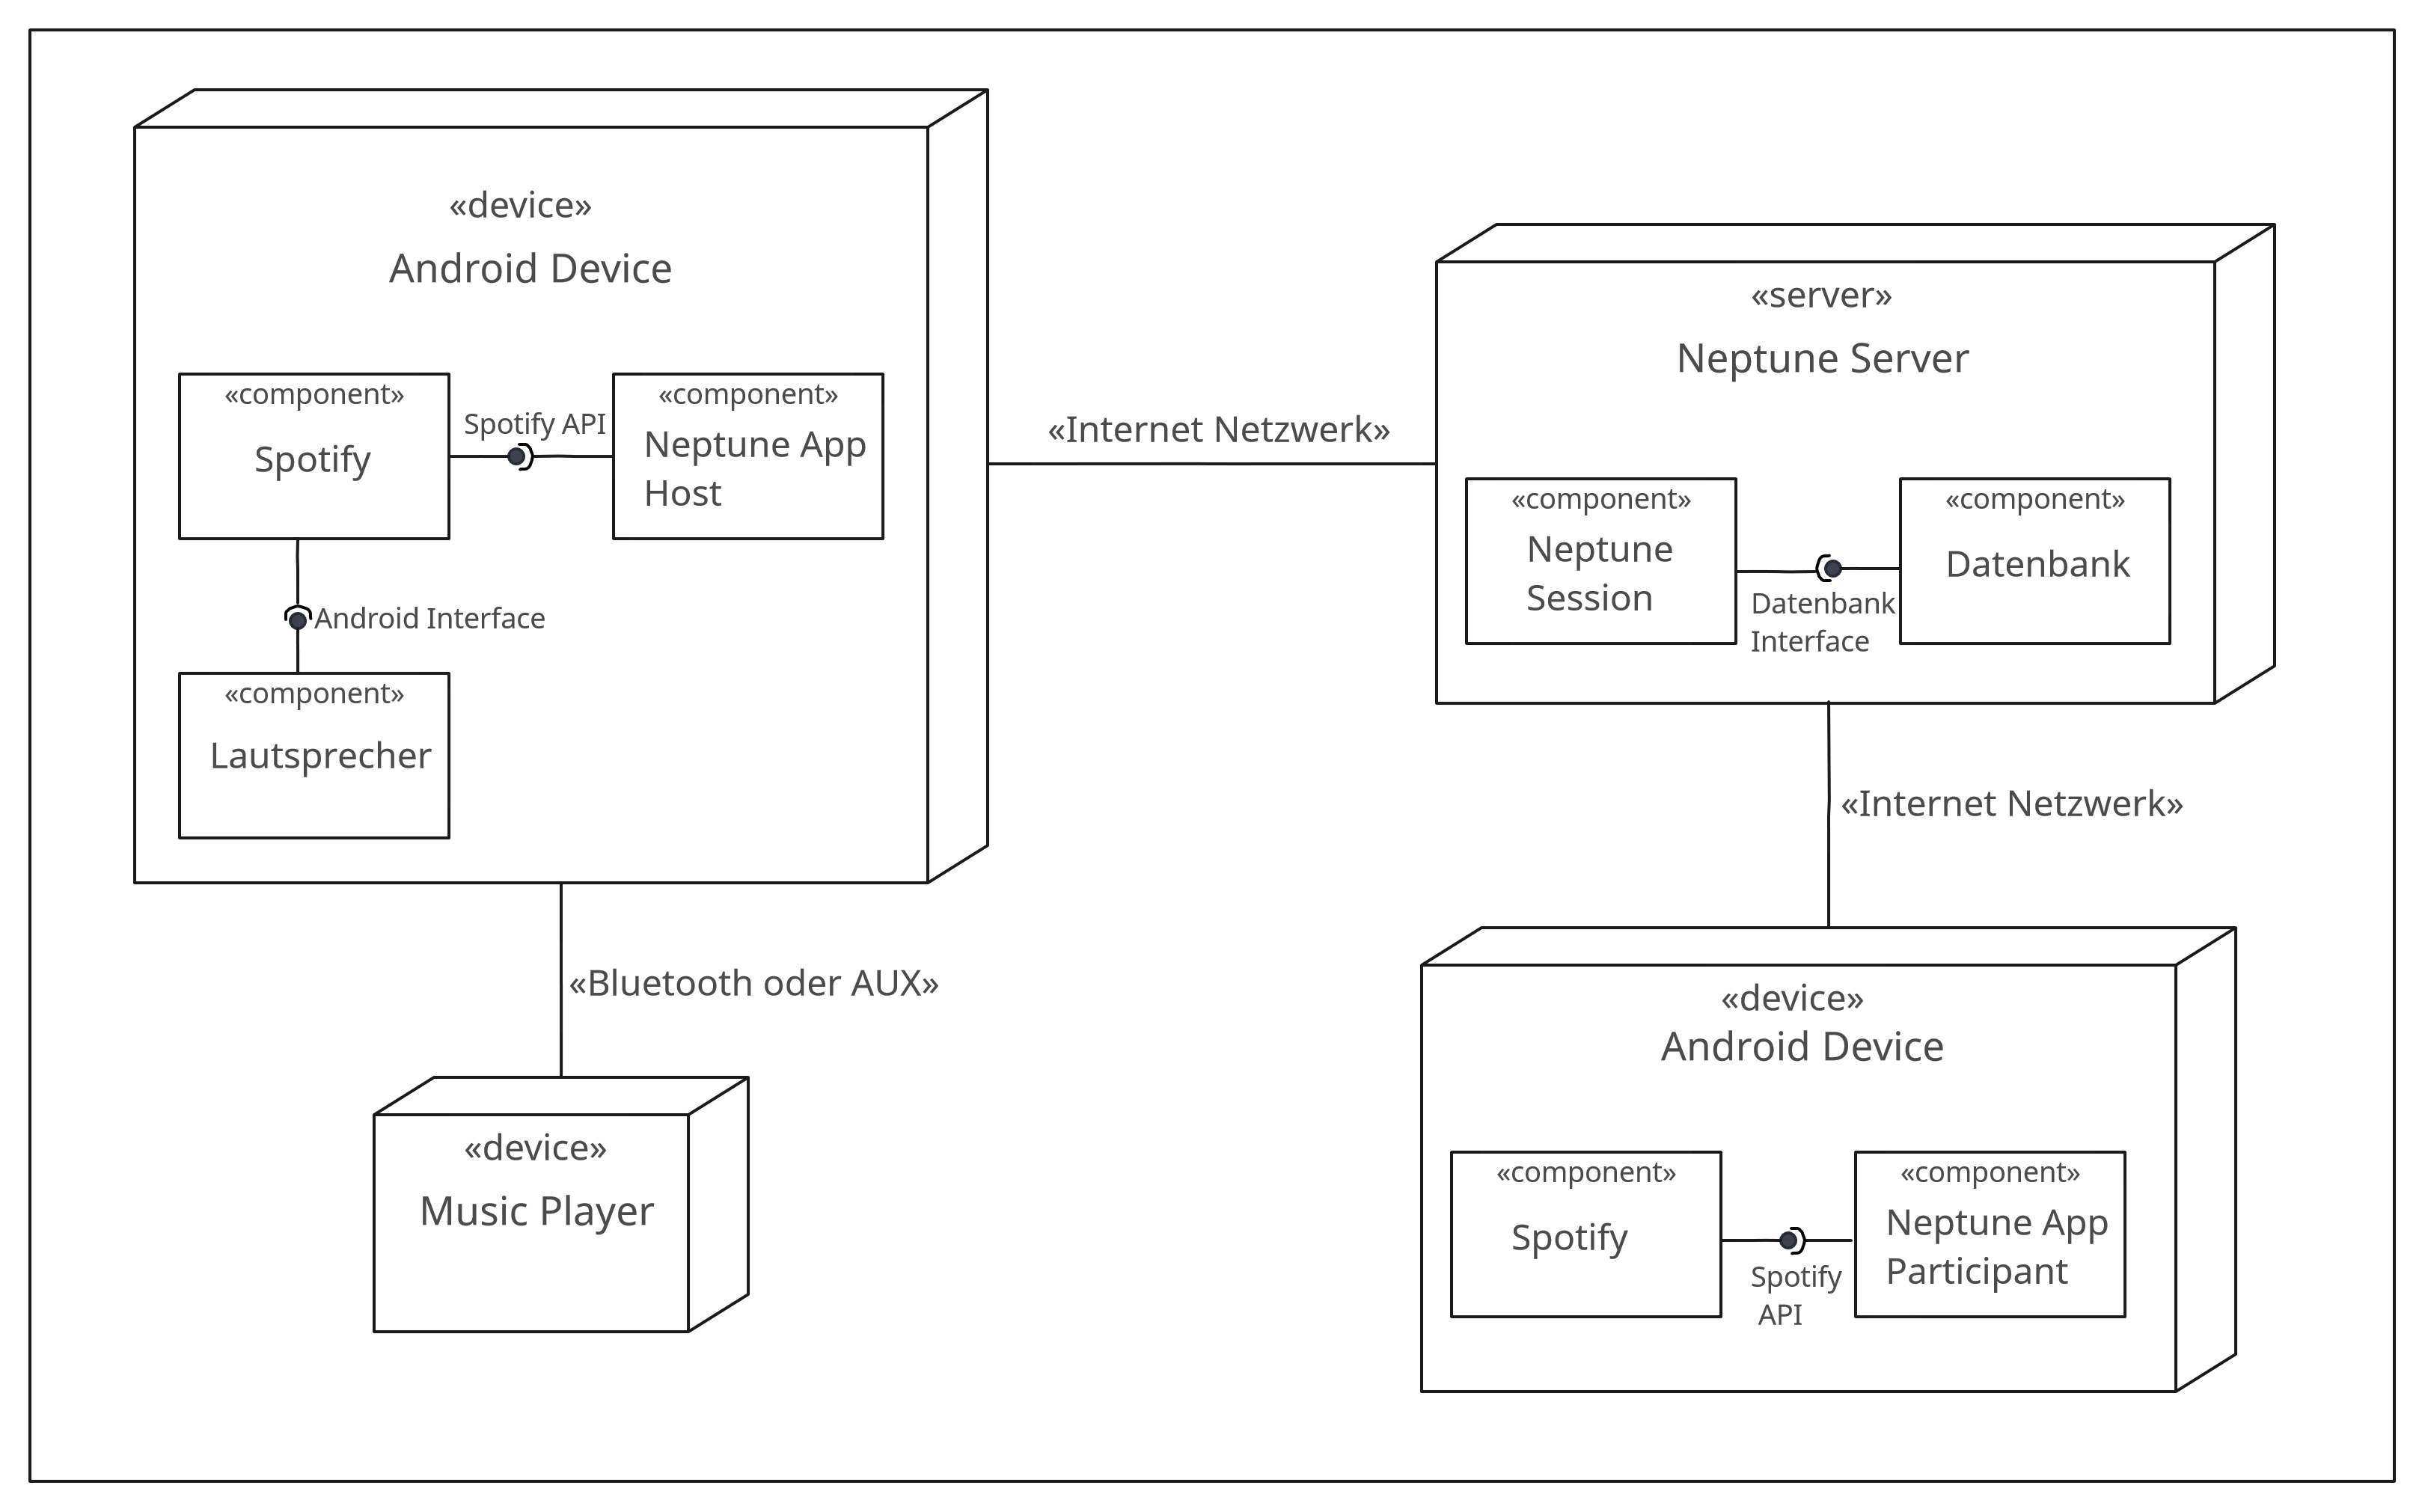
\includegraphics[width = 16cm]{LATEX/Pflichtenheft/GraphicDesigns/Verteilungsdiagramm.png}
    \caption{Verteilungsdiagramm}
    \label{fig:Verteilungsdiagramm}
\end{figure}


\chapter{Benutzeroberfläche}
\label{chap:Benutzeroberfläche}

\section{Einführung}
\label{sec:Benutzeroberfläche:Einführung}
\textbf{} Die Benutzeroberfläche wird so gestaltet, dass diese einfach von Nutzern ohne Vorkenntnissen über die App genutzt werden kann.

\section{Startmenü}
\label{sec:Benutzeroberfläche:Startmenü}
Der Nutzer landet beim Start der App immer im Startmenü.

\section{Participant Ansicht}
\label{sec:Benutzeroberfläche:participantAnsicht}
In der Participant Ansicht kann der Nutzer einer Gruppe beitreten und je nach Modus neue Lieder vorschlagen und liken.

\section{Host Ansicht}
\label{sec:Benutzeroberfläche:hostAnsicht}
In der Host Ansicht kann der Host einen Modus auswählen und Einstellungen für die Session definieren. Des weiteren kann er wie ein Participant Lieder hinzufügen und liken. Zusätzlich kann der Host Lieder aus der Queue löschen und Lieder aus der Vorschlagsliste zur Queue hinzufügen

\section{Grafikentwürfe}
\label{sec:Benutzeroberfläche:Grafikentwürfe}
Um ein übersichtliches Startmenü zu gewährleisten kann der Nutzer nur zwischen den Optionen ''Gruppe beitreten'' und ''Gruppe erstellen'' wählen. 

%
\makeatletter
\setlength{\@fptop}{1cm}
\makeatother
%

\begin{figure}
    \hypertarget{startPage}{}
    \begin{minipage}[t]{7 cm}
        \vspace{-1.5ex}
        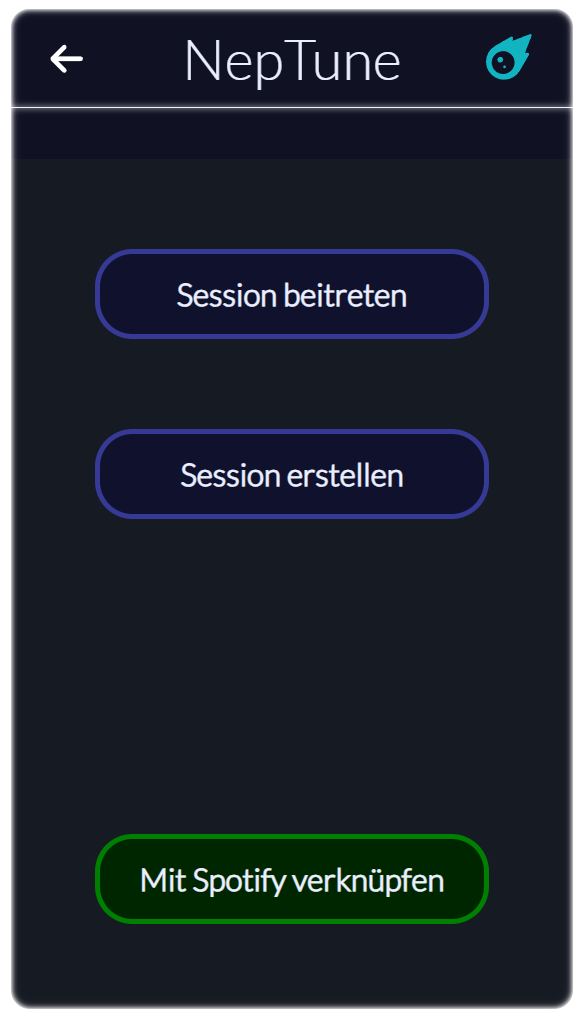
\includegraphics[width=7cm]{LATEX/Pflichtenheft/GraphicDesigns/startPage.png}
        \caption{startPage}
    \end{minipage}
    \hspace{1cm}
    \begin{minipage}[t]{7 cm}
        \vspace{1cm}
        Bei Drücken des Zurück Button erscheint ein Pop-Up Fenster mit der Frage ''NepTune wirklich schließen?''. In diesem Pop-Up kann sich der Nutzer nun zwischen ''Ja'' und ''Nein'' entscheiden. Durch auswählen von ''Ja'' wird die App geschlossen. Durch Auswählen von ''Nein'' bleibt der Nutzer in der \hyperlink{startPage}{startPage}.\\
        Durch klicken des ''Session beitreten" Button gelangt der Nutzer auf die \hyperlink{userJoinGroupPage}{userJoinGroupPage}. \\
        Durch klicken des ''Session erstellen'' Button gelangt der Nutzer auf die \hyperlink{hostModusSelectPage}{hostModusSelectPage}. Der ''Session erstellen'' Button ist jedoch so lange deaktiviert, bis sich der Nutzer mit über den ''Mit Spotify verknüpfen'' Button mit Spotify verbunden hat und verifiziert wurde, dass es sich um einen Spotify Premium Account handelt.\\
        Hat sich der Nutzer mit Spotify angemeldet, so ändert sich der ''Mit Spotify verknüpfen'' Button zu ''Von Spotify trennen''. Durch Nutzung des Buttons wird das Spotify Konto des Nutzers wieder von NepTune getrennt.
    \end{minipage}
\end{figure}

\begin{figure}
    \hypertarget{userJoinGroupPage}{}
    \begin{minipage}[t]{7 cm}
        \vspace{-1.5ex}
        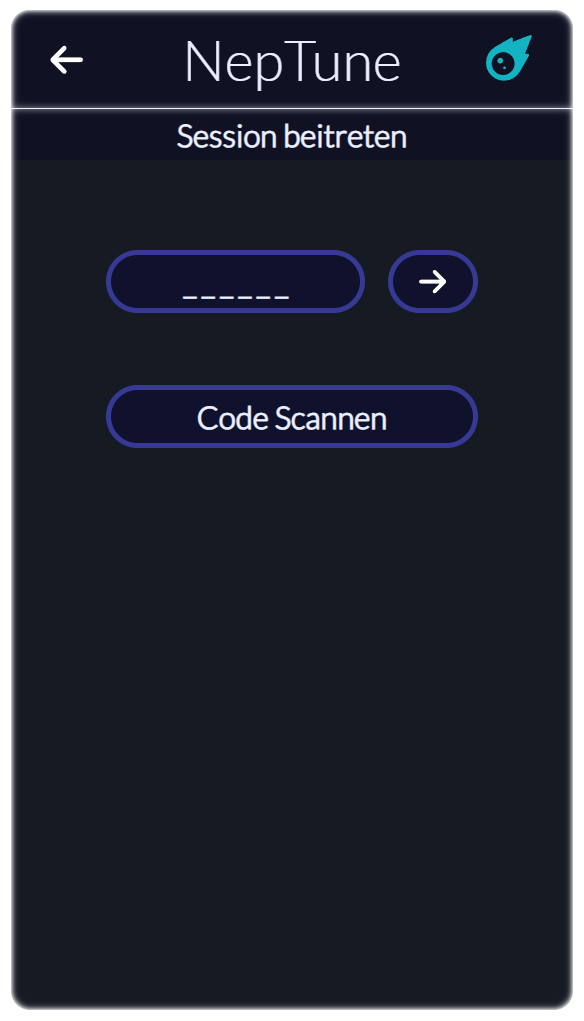
\includegraphics[width=7cm]{LATEX/Pflichtenheft/GraphicDesigns/userJoinGroupPage.png}
        \caption{userJoinGroupPage}
    \end{minipage}
    \hspace{1cm}
    \begin{minipage}[t]{7 cm}
        \vspace{1cm}
         Der <- Button oben links führt zurück auf die \hyperlink{startPage}{startPage}.
         Im Textfeld darunter kann der 6-stellige Zugangscode eingegeben werden. Existiert eine Session zu dem eingegeben Zugangscode kann man mit dem -> Button zur
         \hyperlink{userVotePage}{userVotePage} springen. Alternativ kann mit dem ''Code Scannen'' Button den QR-Codereader öffnen. Nach erfolgreichen einscannen landet man hier ebenfalls auf der \hyperlink{userVotePage}{userVotePage}. 
         
    \end{minipage}
\end{figure}

\begin{figure}
    \hypertarget{userVotePage}{}
    \begin{minipage}[t]{7 cm}
        \vspace{-1.5ex}
        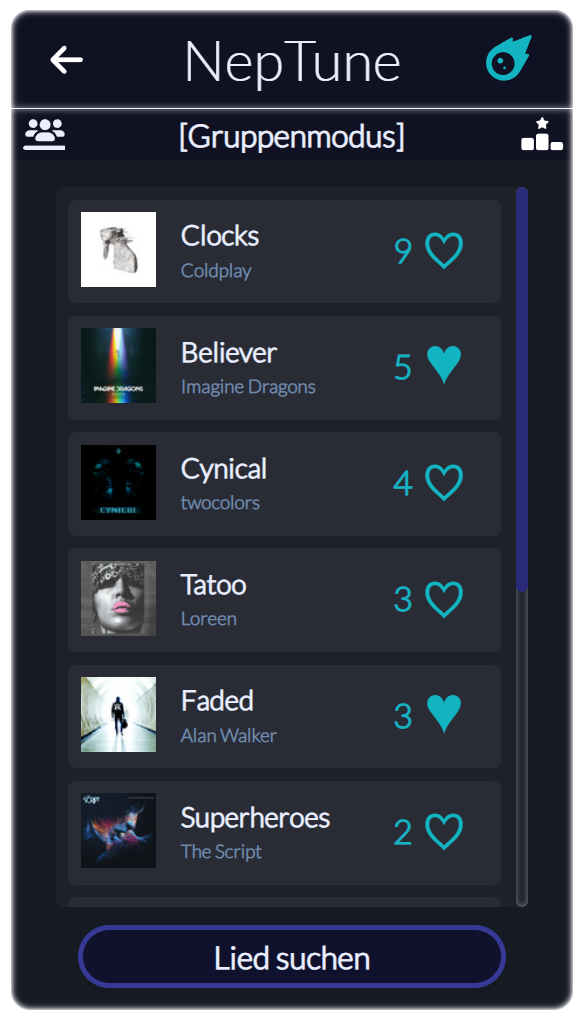
\includegraphics[width=7cm]{LATEX/Pflichtenheft/GraphicDesigns/userVotePage.png}
        \caption{userVotePage}
    \end{minipage}
    \hspace{1cm}
    \begin{minipage}[t]{7 cm}
        \vspace{1cm}
        Auf der userVotingPage sieht der Nutzer die Tracks die bereits von Sessionmitglieder upgevotet wurden. Zudem kann er Lieder upvoten, die er noch nicht upgevotet hat, durch erneutes Anklicken wird der Upvote wieder entfernt. Durch drücken des ''Lied suchen'' Button springt man in die  \hyperlink{userSearchPage}{userSearchPage}. Über den Zurück-Knopf oben links gelangt der Nutzer zurück zur \hyperlink{startPage}{startPage}. Dieser Vorgang muss über ein Pop-Up Fenster bestätigt werden, da gleichseitig die Gruppe verlassen wird.
    \end{minipage}
\end{figure}

\begin{figure}
    \hypertarget{userSearchPage}{}
    \begin{minipage}[t]{7 cm}
        \vspace{-1.5ex}
        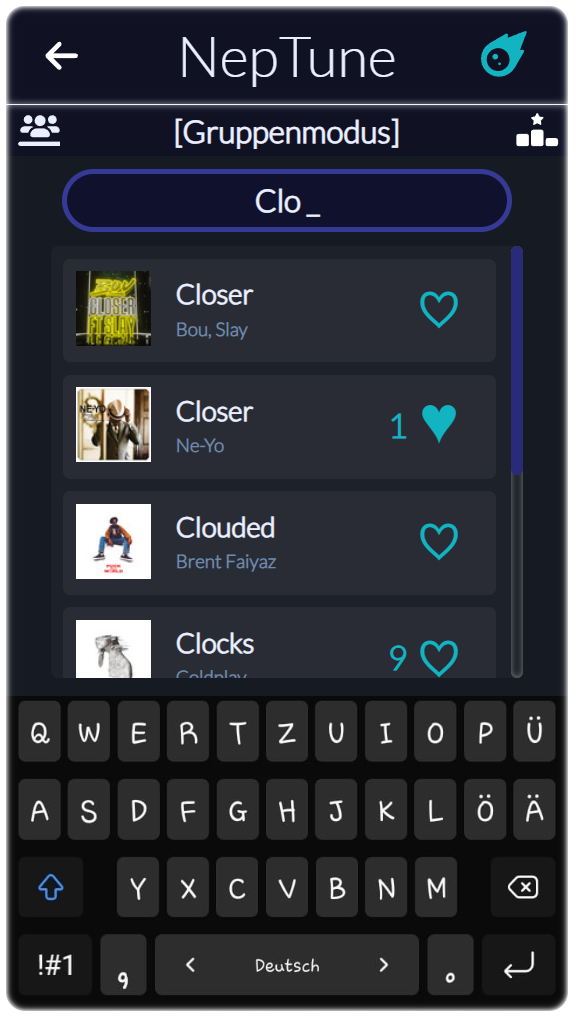
\includegraphics[width=7cm]{LATEX/Pflichtenheft/GraphicDesigns/userSearchPage.png}
        \caption{userSearchPage}
    \end{minipage}
    \hspace{1cm}
    \begin{minipage}[t]{7 cm}
        \vspace{1cm}
        Der <- Button führt zurück in die \hyperlink{userVotingPage}{userVotingPage}  
    \end{minipage}
\end{figure}

\begin{figure}
    \hypertarget{hostModusSelectPage}{}
    \begin{minipage}[t]{7 cm}
        \vspace{-1.5ex}
        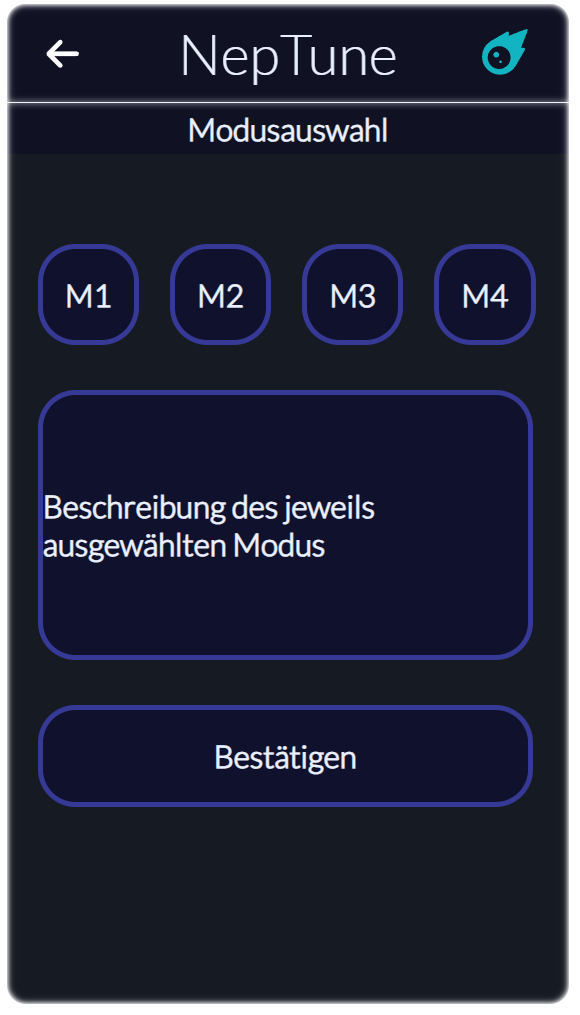
\includegraphics[width=7cm]{LATEX/Pflichtenheft/GraphicDesigns/hostModusSelectPage.png}
        \caption{hostModusSelectPage}
    \end{minipage}
    \hspace{1cm}
    \begin{minipage}[t]{7 cm}
        \vspace{1cm}
        In der Modusauswahlview kann der Host einen der vier möglichen Modi auswählen, dabei ist am Beginn ist der General Mode ausgewählt. Im Textfeld darunter wird ein kurze Beschreibung des gerade ausgewählten Modus angezeigt. Mit dem Bestätigen Button springt man in die Einstellungspage des Hosts.
    \end{minipage}
\end{figure}

\begin{figure}
    \hypertarget{hostModusSettingsPage}{}
    \begin{minipage}[t]{7 cm}
        \vspace{-1.5ex}
        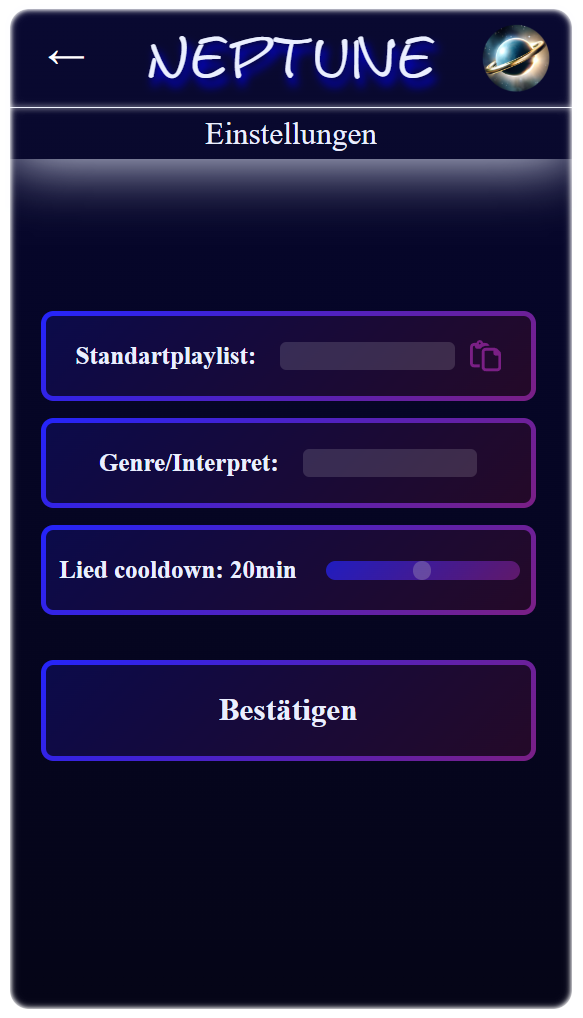
\includegraphics[width=7cm]{LATEX/Pflichtenheft/GraphicDesigns/hostModusSettingsPage.png}
        \caption{hostModusSettingsPage}
    \end{minipage}
    \hspace{1cm}
    \begin{minipage}[t]{7 cm}
        \vspace{1cm}
        In den Host Einstellungen kann man mit dem Einfügen eines Spotifyplaylistlinkes eine Standartplaylist hinterlegen.
        In der Genre/Artist Feld kann man die Genre und Artistbeschränkungen auswählen \textit{(Todo wie)}
    \end{minipage}
\end{figure}

\begin{figure}
    \hypertarget{hostControlPage}{}
    \begin{minipage}[t]{7 cm}
        \vspace{-1.5ex}
        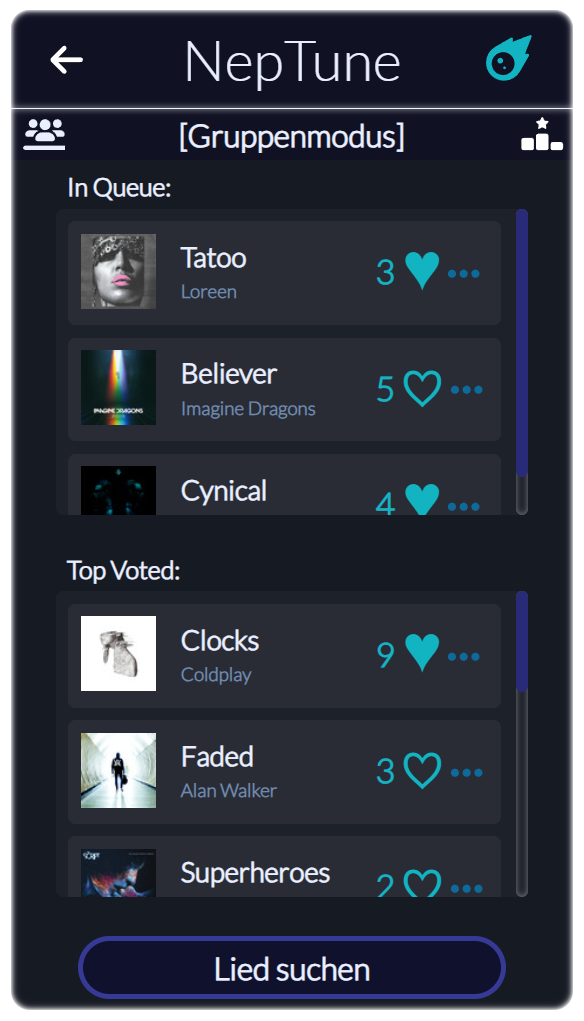
\includegraphics[width=7cm]{LATEX/Pflichtenheft/GraphicDesigns/hostControlPage.png}
        \caption{hostControlPage}
    \end{minipage}
    \hspace{1cm}
    \begin{minipage}[t]{7 cm}
        \vspace{1cm}
        In der HostControlPage kann der Host die Queue in Spotify einsehen. Genau wie ein Participant kann er hier Upvotes auf Tracks verteilen und wieder entfernen. Zudem kann der Host durch drücken auf die drei Punkte eines Tracks weitere Einstellung vornehmen. Zu diesen gehören das Hinzufügen und Entfernen eines Tracks zur Queue, sowie das Sperren und Entsperren von Tracks. Gesperrte Tracks können keine Upvotes erhalten und werden nicht abgespielt.
    \end{minipage}
\end{figure}

\begin{figure}
    \hypertarget{hostSearchPage}{}
    \begin{minipage}[t]{7 cm}
        \vspace{-1.5ex}
        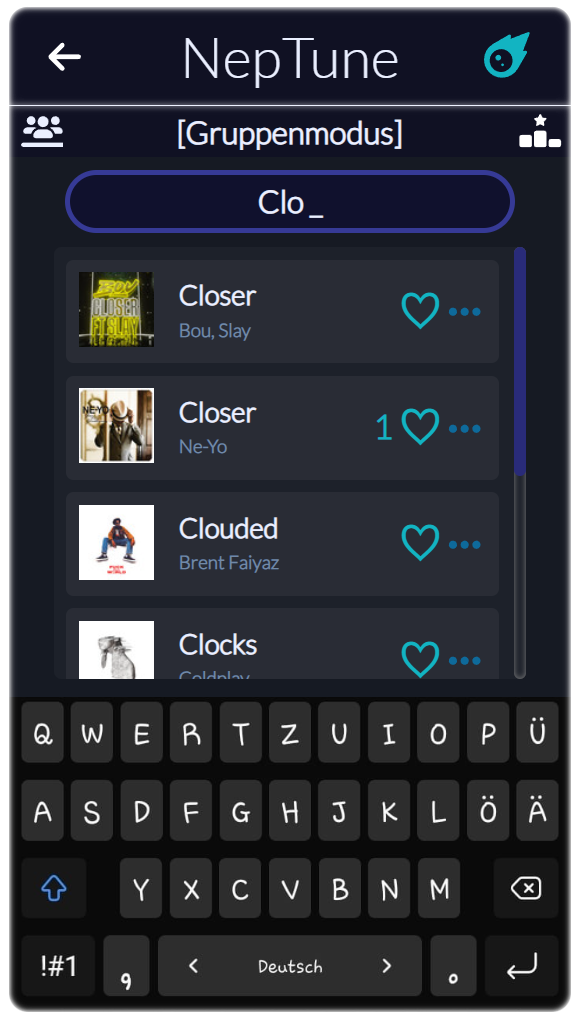
\includegraphics[width=7cm]{LATEX/Pflichtenheft/GraphicDesigns/hostSearchPage.png}
        \caption{hostSearchPage}
    \end{minipage}
    \hspace{1cm}
    \begin{minipage}[t]{7 cm}
        \vspace{1cm}
        TODO
    \end{minipage}
\end{figure}

\begin{figure}
    \hypertarget{shareLinkPopUpPage}{}
    \begin{minipage}[t]{7 cm}
        \vspace{-1.5ex}
        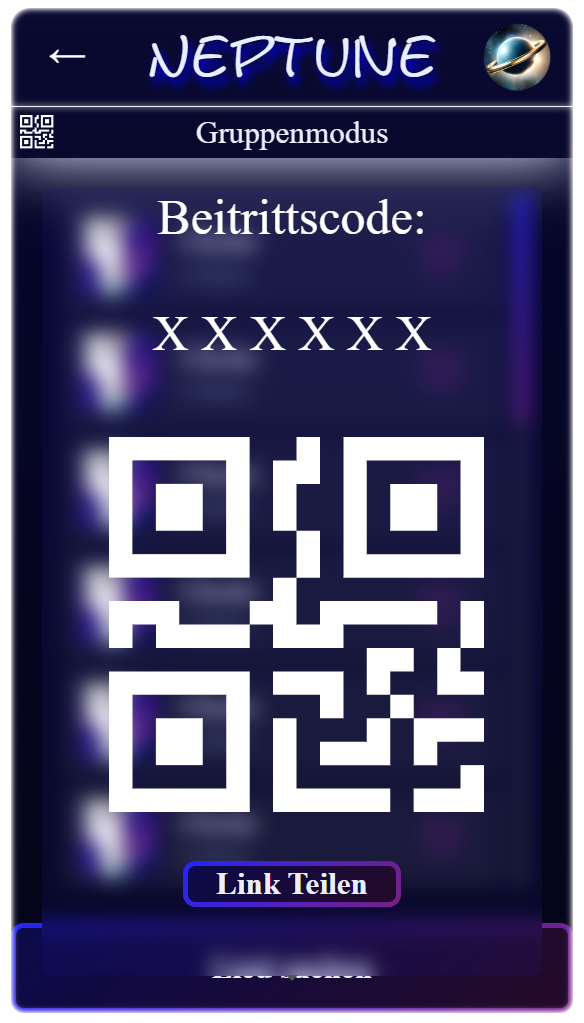
\includegraphics[width=7cm]{LATEX/Pflichtenheft/GraphicDesigns/shareLinkPopUpPage.png}
        \caption{shareLinkPopUpPage}
    \end{minipage}
    \hspace{1cm}
    \begin{minipage}[t]{7 cm}
        \vspace{1cm}
        Die shareLinkPopUpPage stellt für den Host einer Session in gebündelter Form Möglichkeiten zur Verfügung,  User als Participants zu der entsprechenden Session einzuladen. Primär stehen hierfür ein der Session eindeutig zugeordneter, sechstelliger Code aus Ganzzahlen sowie ein analog der Session zugeordneter Beitrittslink zur Verfügung. Für den Beitrittslink ist in der Anzeige ein Button enthalten, mithilfe dessen der Link geteilt werden kann. Für das Teilen wird hierbei die von Android bereitgestellte Schnittfläche verwendet. Darüber hinaus soll als Alternative gleichzeitig auch ein analog funktionierender QR-Code zur Verfügung stehen, welcher in dieser Ansicht mit angezeigt wird. Zusätzlich werden in dieser Anzeige der Bezeichner des Gruppenmodus der Session sowie gegebenenfalls Informationen über Modusseitige Einschränkungen hinsichtlich Genres und Artists angezeigt. Durch Auswahl des "Zurück
 Buttons (symbolisiert durch Pfeil) gelangt man zur zuvor angezeigten Ansicht zurück. Durch Auswahl des "X"-Buttons lässt sich diese Anzeige schließen und man gelangt zur \textit{(uv)-}Ansicht. \textit{(TODO: ENTSPRECHENDE ANSICHT DAZU SCHREIBEN!)}
 \end{minipage}
\end{figure}

\begin{figure}
    \hypertarget{statisticsPopUpPage}{}
    \begin{minipage}[t]{7 cm}
        \vspace{-1.5ex}
        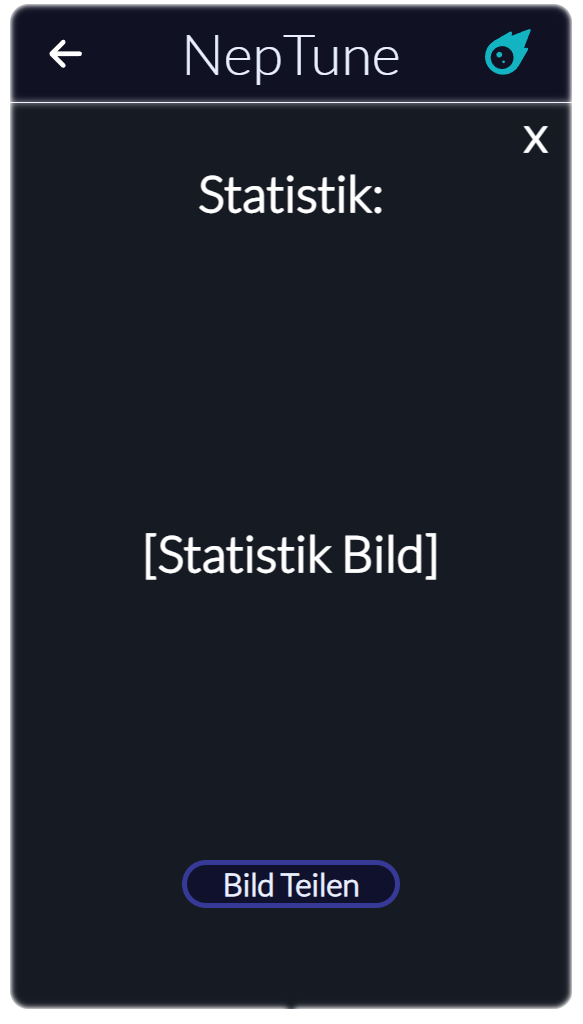
\includegraphics[width=7cm]{LATEX/Pflichtenheft/GraphicDesigns/statisticsPopUpPage.png}
        \caption{statisticsPopUpPage}
    \end{minipage}
    \hspace{1cm}
    \begin{minipage}[t]{7 cm}
        \vspace{1cm}
        TODO
    \end{minipage}
\end{figure}

\chapter{Qualitätszielbestimmungen}
\label{chap:Qualitätszielbestimmungen}

\textbf{Korrekte Funktionalität}: Die korrekte Funktionalität der App muss gewährleistet sein. Maßgeblich zur Definition dieser korrekten Funktionalität ist dieses Pflichtenheft und insbesondere die Musskriterien aus dem Kapitel der Zielbestimmungen (Kapitel \ref{sec:Zielbestimmungen:Musskriterien}).

\textbf{Benutzerfreundlichkeit}: Die App soll eine einfache und intuitive Benutzererfahrung bieten. Die Navigation innerhalb der App soll für alle Benutzer leicht verständlich sein, ohne dass diese eine Einführung in die App-Bedienung benötigen. Das maßgebliche Kriterium dafür ist, dass Benutzer der Zielgruppe (Kapitel \ref{sec:Einleitung:Zielgruppe}) die App bei der ersten Benutzung innerhalb von zwei Minuten problemlos navigieren können laut eigener Einschätzung. (AUßER LIKE UND ZURÜCK; HÖCHSTENS 3 BUTTONS; AUßGENOMEN HOST IN SEINER VIEW -> DORT 5 BUTTONS)

\textbf{Schnelligkeit}: Die App soll durch Reaktionsschnelligkeit ein flüssiges und ansprechendes Nutzungserlebnis ermöglichen. Das maßgebliche Kriterium dafür ist, dass jede Schaltflächenbedienung ein unmittelbares Feedback innerhalb von 300ms für den Benutzer auslöst, ohne dass dieser eine Wartezeit bemerkt, solange das Endgerät hinreichend aktuell ist. Hinreichend aktuell sind dabei insbesondere Geräte, die weniger als ein Jahr alt sind und die aktuellste verfügbare Betriebssystemversion installiert haben.

\textbf{Sicherheit der Benutzerdaten}: Es ist essentiell, dass die persönlichen Daten der Benutzer geschützt sind. Jegliche Interaktion mit und Datenverarbeitung durch die App muss datenschutzkonform sein und Datensicherheit bieten. Maßgeblich ist dafür die gesetzliche Regelung.

\textbf{Stabilität und Zuverlässigkeit}: Die App muss robust sein und selbst unter Last und bei mäßig vielen gleichzeitigen Benutzern stabil bleiben, sodass Abstürze oder unerwartete Fehler weitestgehend vermieden werden. Das maßgebliche Kriterium dafür sind die Testszenarien mit zahlreichen gleichzeitigen Usern. (solche Tests auch einfügen !!!)

\textbf{Wartbarkeit und Portierungsmöglichkeiten}: Die Architektur der App soll gut wartbar sein, um zukünftige Anpassungen oder Erweiterungen zu ermöglichen. Zudem soll die Architektur die Möglichkeit zur verhältnismäßig einfachen Portierung der App auf andere mobile Betriebssysteme wie iOS bieten. Dazu soll möglichst viel Logik auf dem Server geschehen, wie im Systemmodell beschrieben (Kapitel \ref{chap:Systemmodell}). Für diese Qualitätszielbestimmung existiert absichtlich kein gerichtsfestes Kriterium zur Überprüfung, maßgeblich ist die subjektive Einschätzung von Betrachtern des Systems. Die Erfüllung dieser Qualitätszielbestimmung ist im Verhältnis zu den anderen Bestimmungen nachrangig. (NACHFRAGEN OB OK?)

\textbf{Grundsätzliches zur Qualität}: Diese Qualitätszielbestimmungen werden während allen Projektphasen beachtet und in der Qualitätssicherungsphase intern abgenommen. Die Qualität der App besitzt während allen Projektphasen einen sehr hohen Stellenwert: Sie wird stets als Priorität betrachtet und in der Qualitätssicherungsphase abschließend und eingehend geprüft.



\chapter{Anwendungsfälle}
\label{chap:Anwendungsfälle}

In diesem Kapitel werden einige Anwendungsfälle der App mithilfe von Use Case Diagrammen anschaulich gemacht. Diese beschreiben das Starten einer Session, sowie die einzelnen Modi der App.

\section{Session erstellen}
\label{sec:Anwendungsfälle:Session erstellen}

\begin{figure}[h]
   \hypertarget{Anwendungsfaelle}{}
    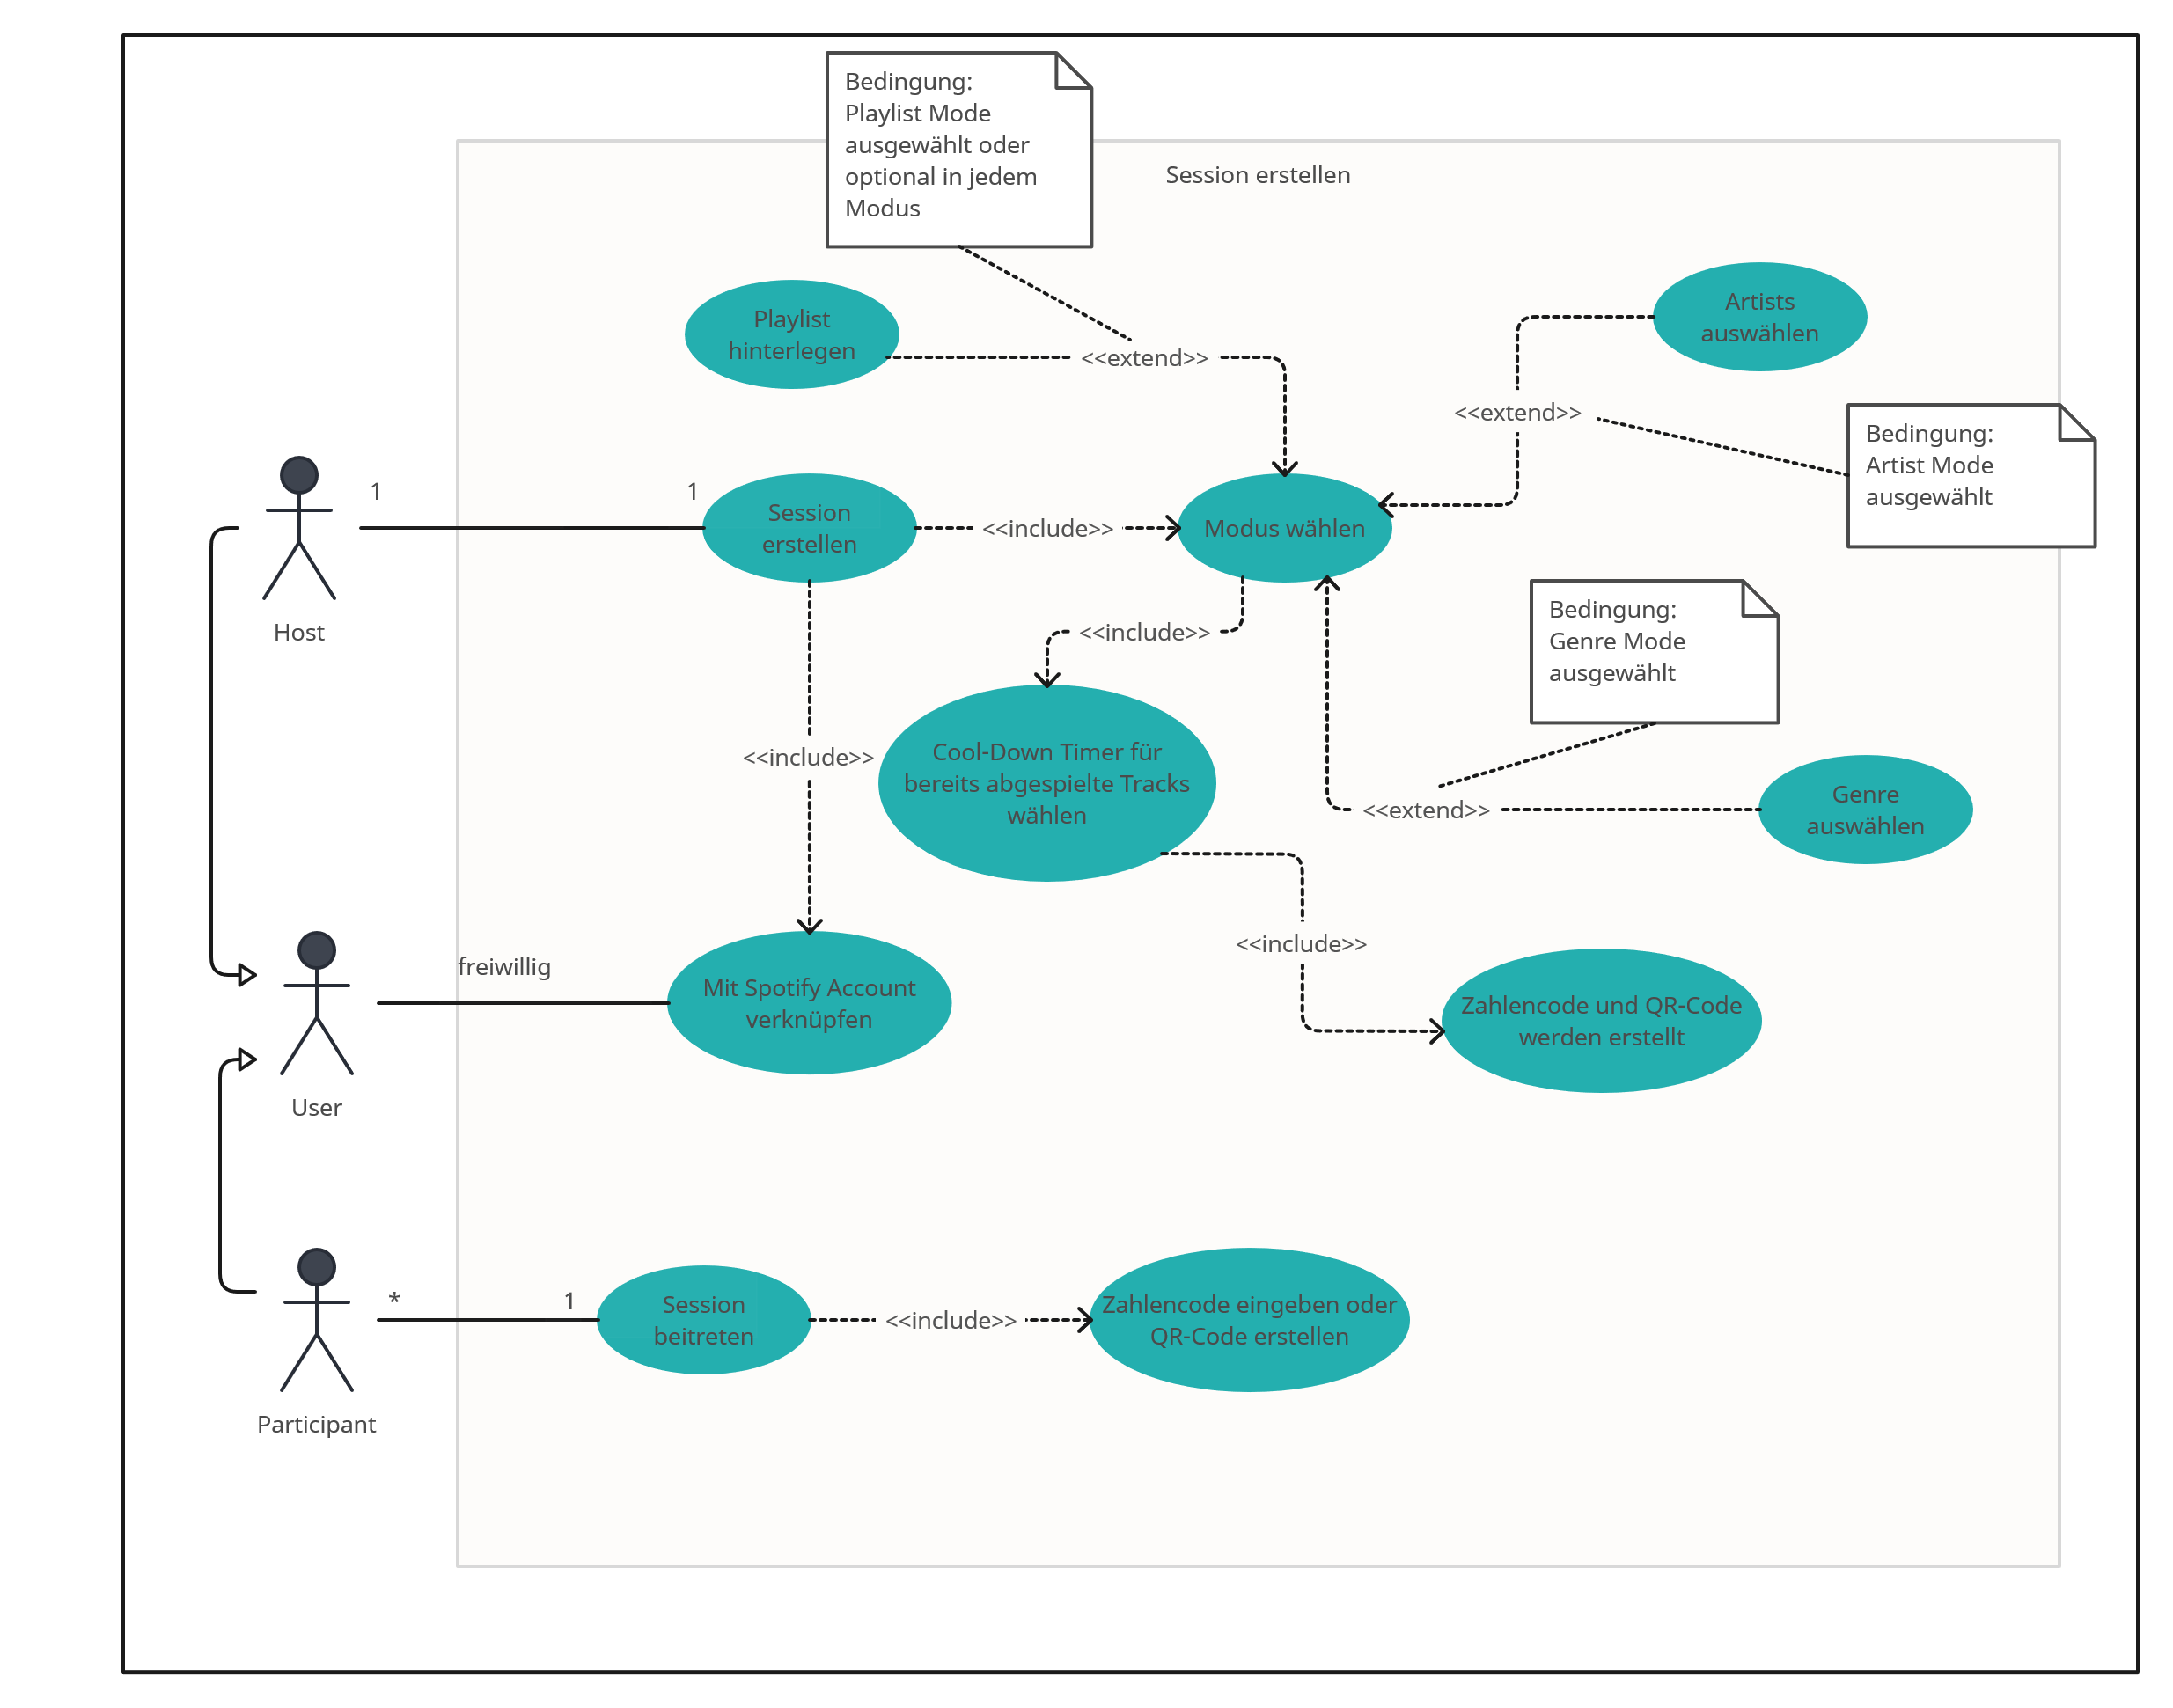
\includegraphics[width = 16cm]{LATEX/Pflichtenheft/GraphicDesigns/Use Case Session erstellen.png}
    \caption{Session erstellen}
    \label{fig:Use Case App Start}
\end{figure}

\newpage

\section{General Mode}
\label{sec:Anwendungsfälle:General Mode}

\begin{figure}[h]
    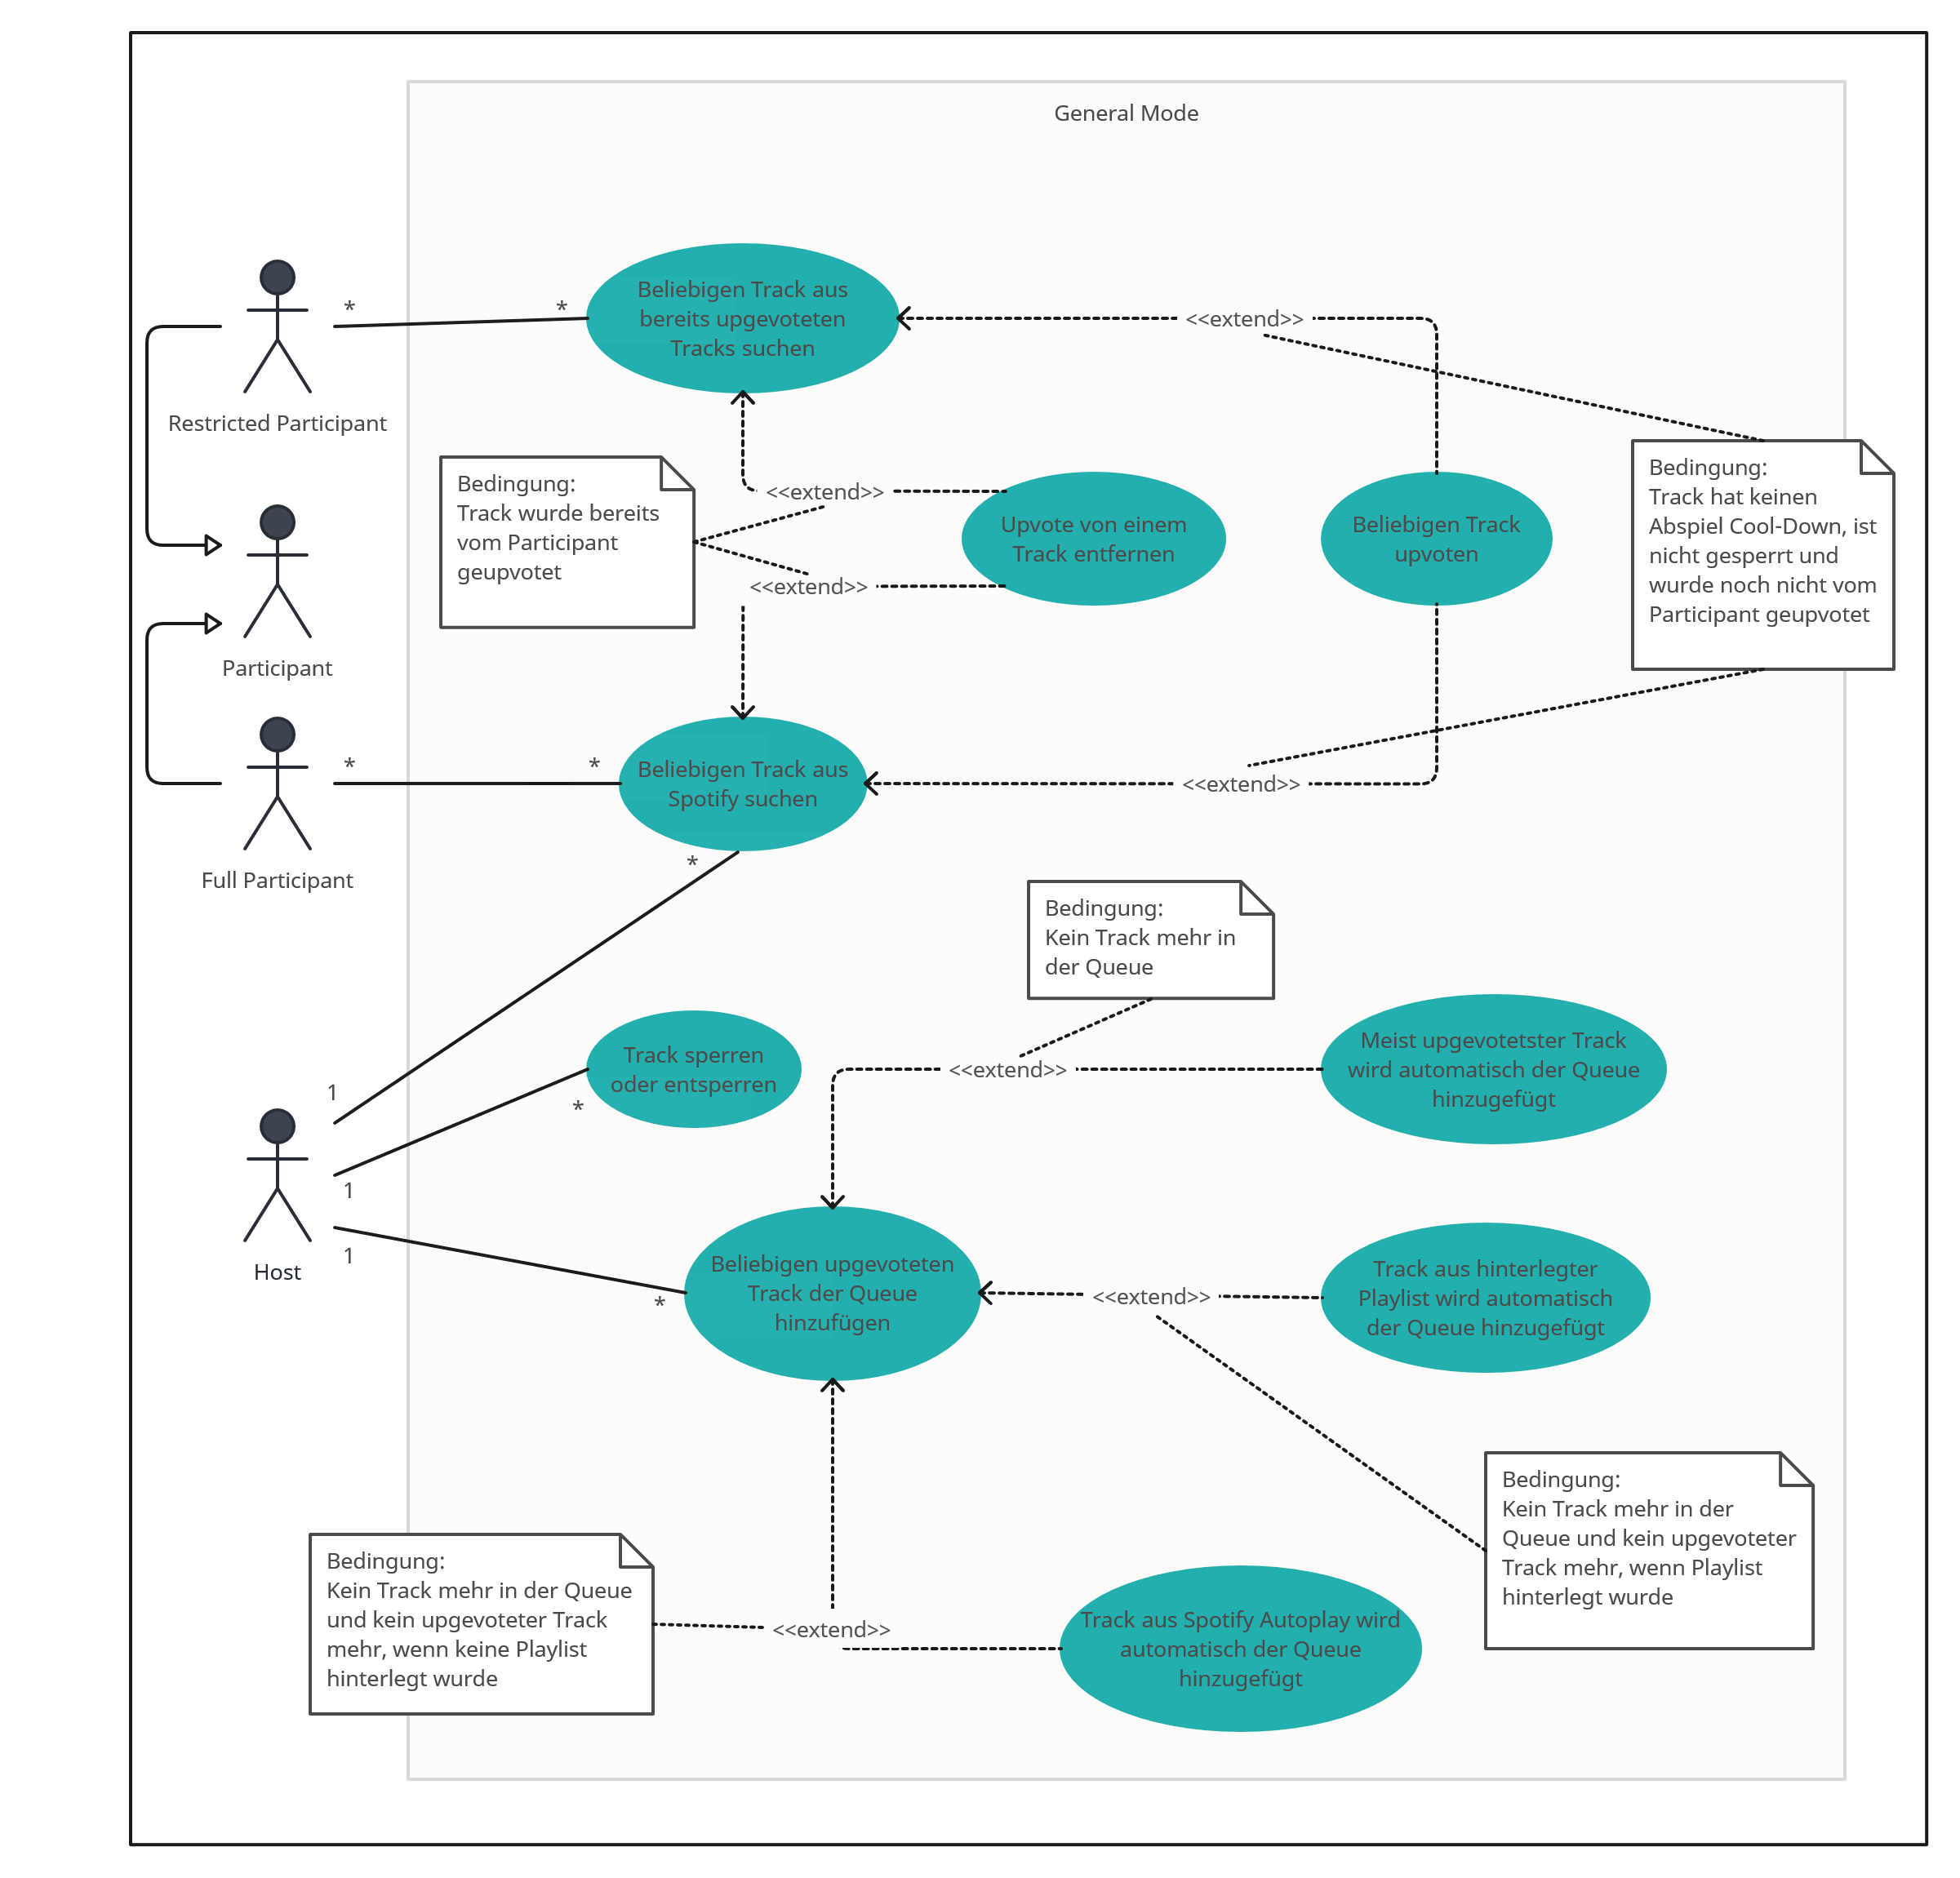
\includegraphics[width = 16cm]{LATEX/Pflichtenheft/GraphicDesigns/Use Case General Mode.png}
    \caption{General Mode}
    \label{fig:Use Case General Mode}
\end{figure}

\newpage

\section{Artist Mode}
\label{sec:Anwendungsfälle:Artist Mode}

\begin{figure}[h]
    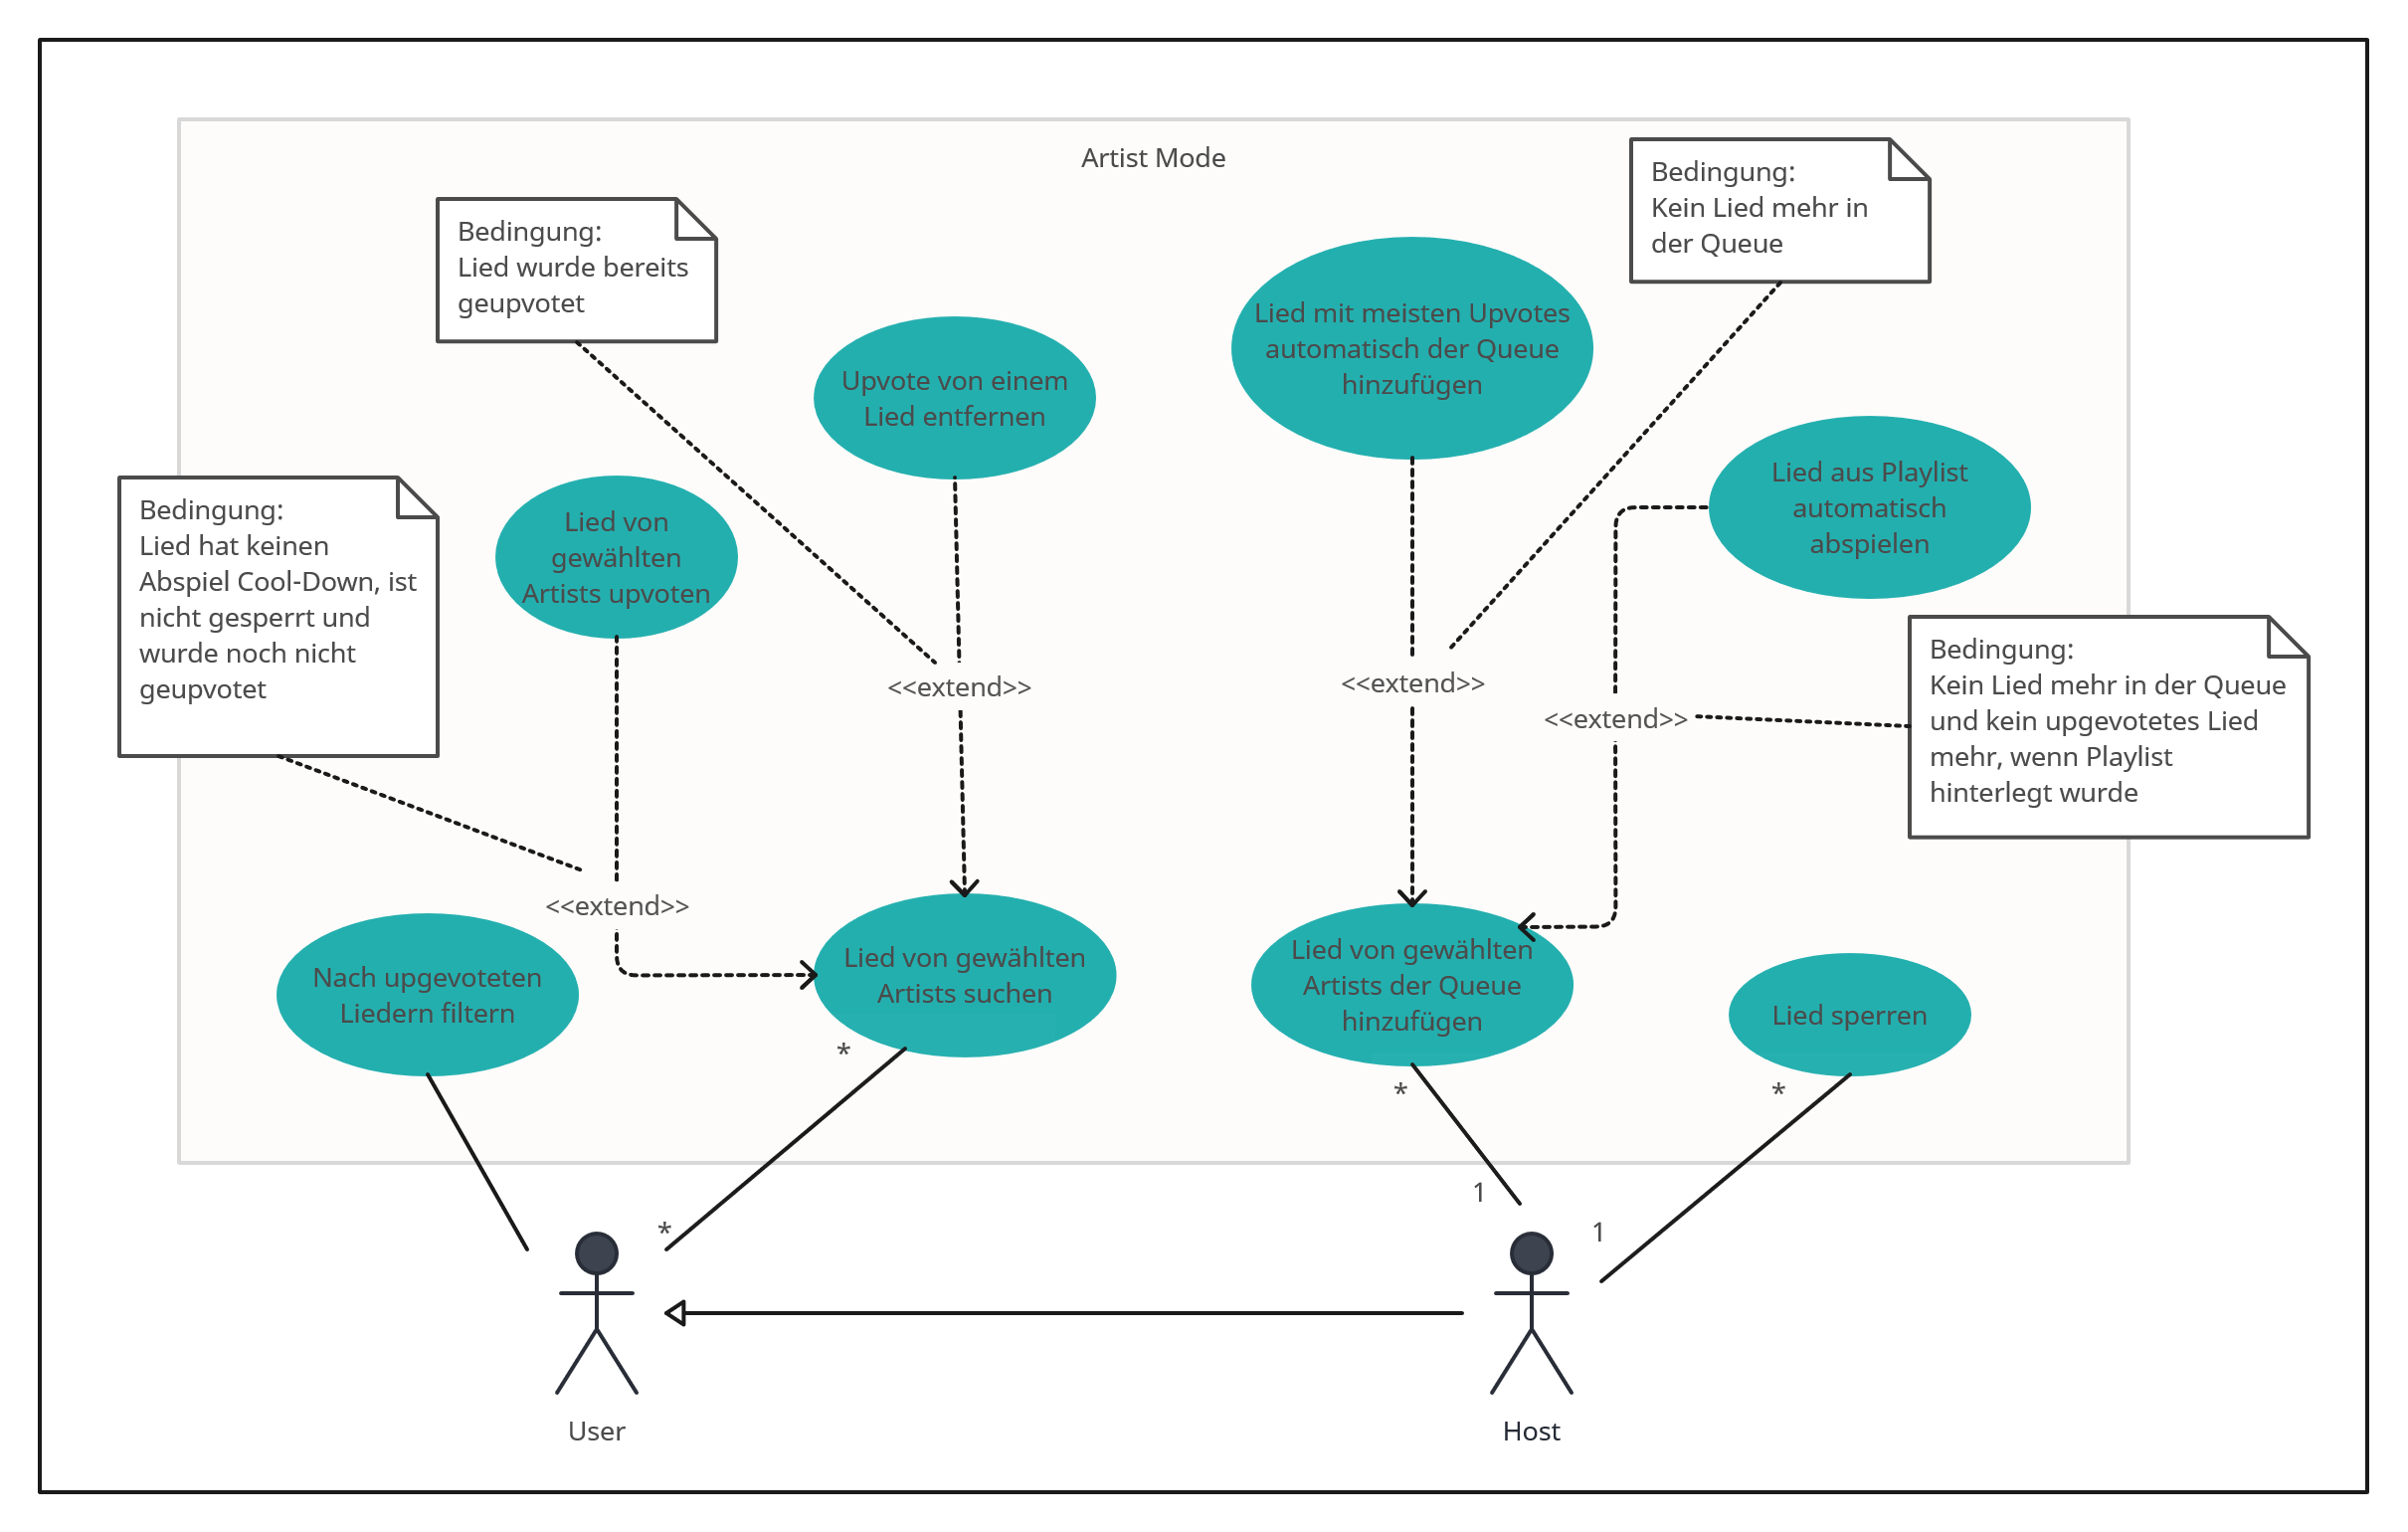
\includegraphics[width = 16cm]{LATEX/Pflichtenheft/GraphicDesigns/Use Case Artist Mode.png}
    \caption{Artist Mode}
    \label{fig:Use Case Artist Mode}
\end{figure}

\newpage

\section{Genre Mode}
\label{sec:Anwendungsfälle:Genre Mode}

\begin{figure}[h]
    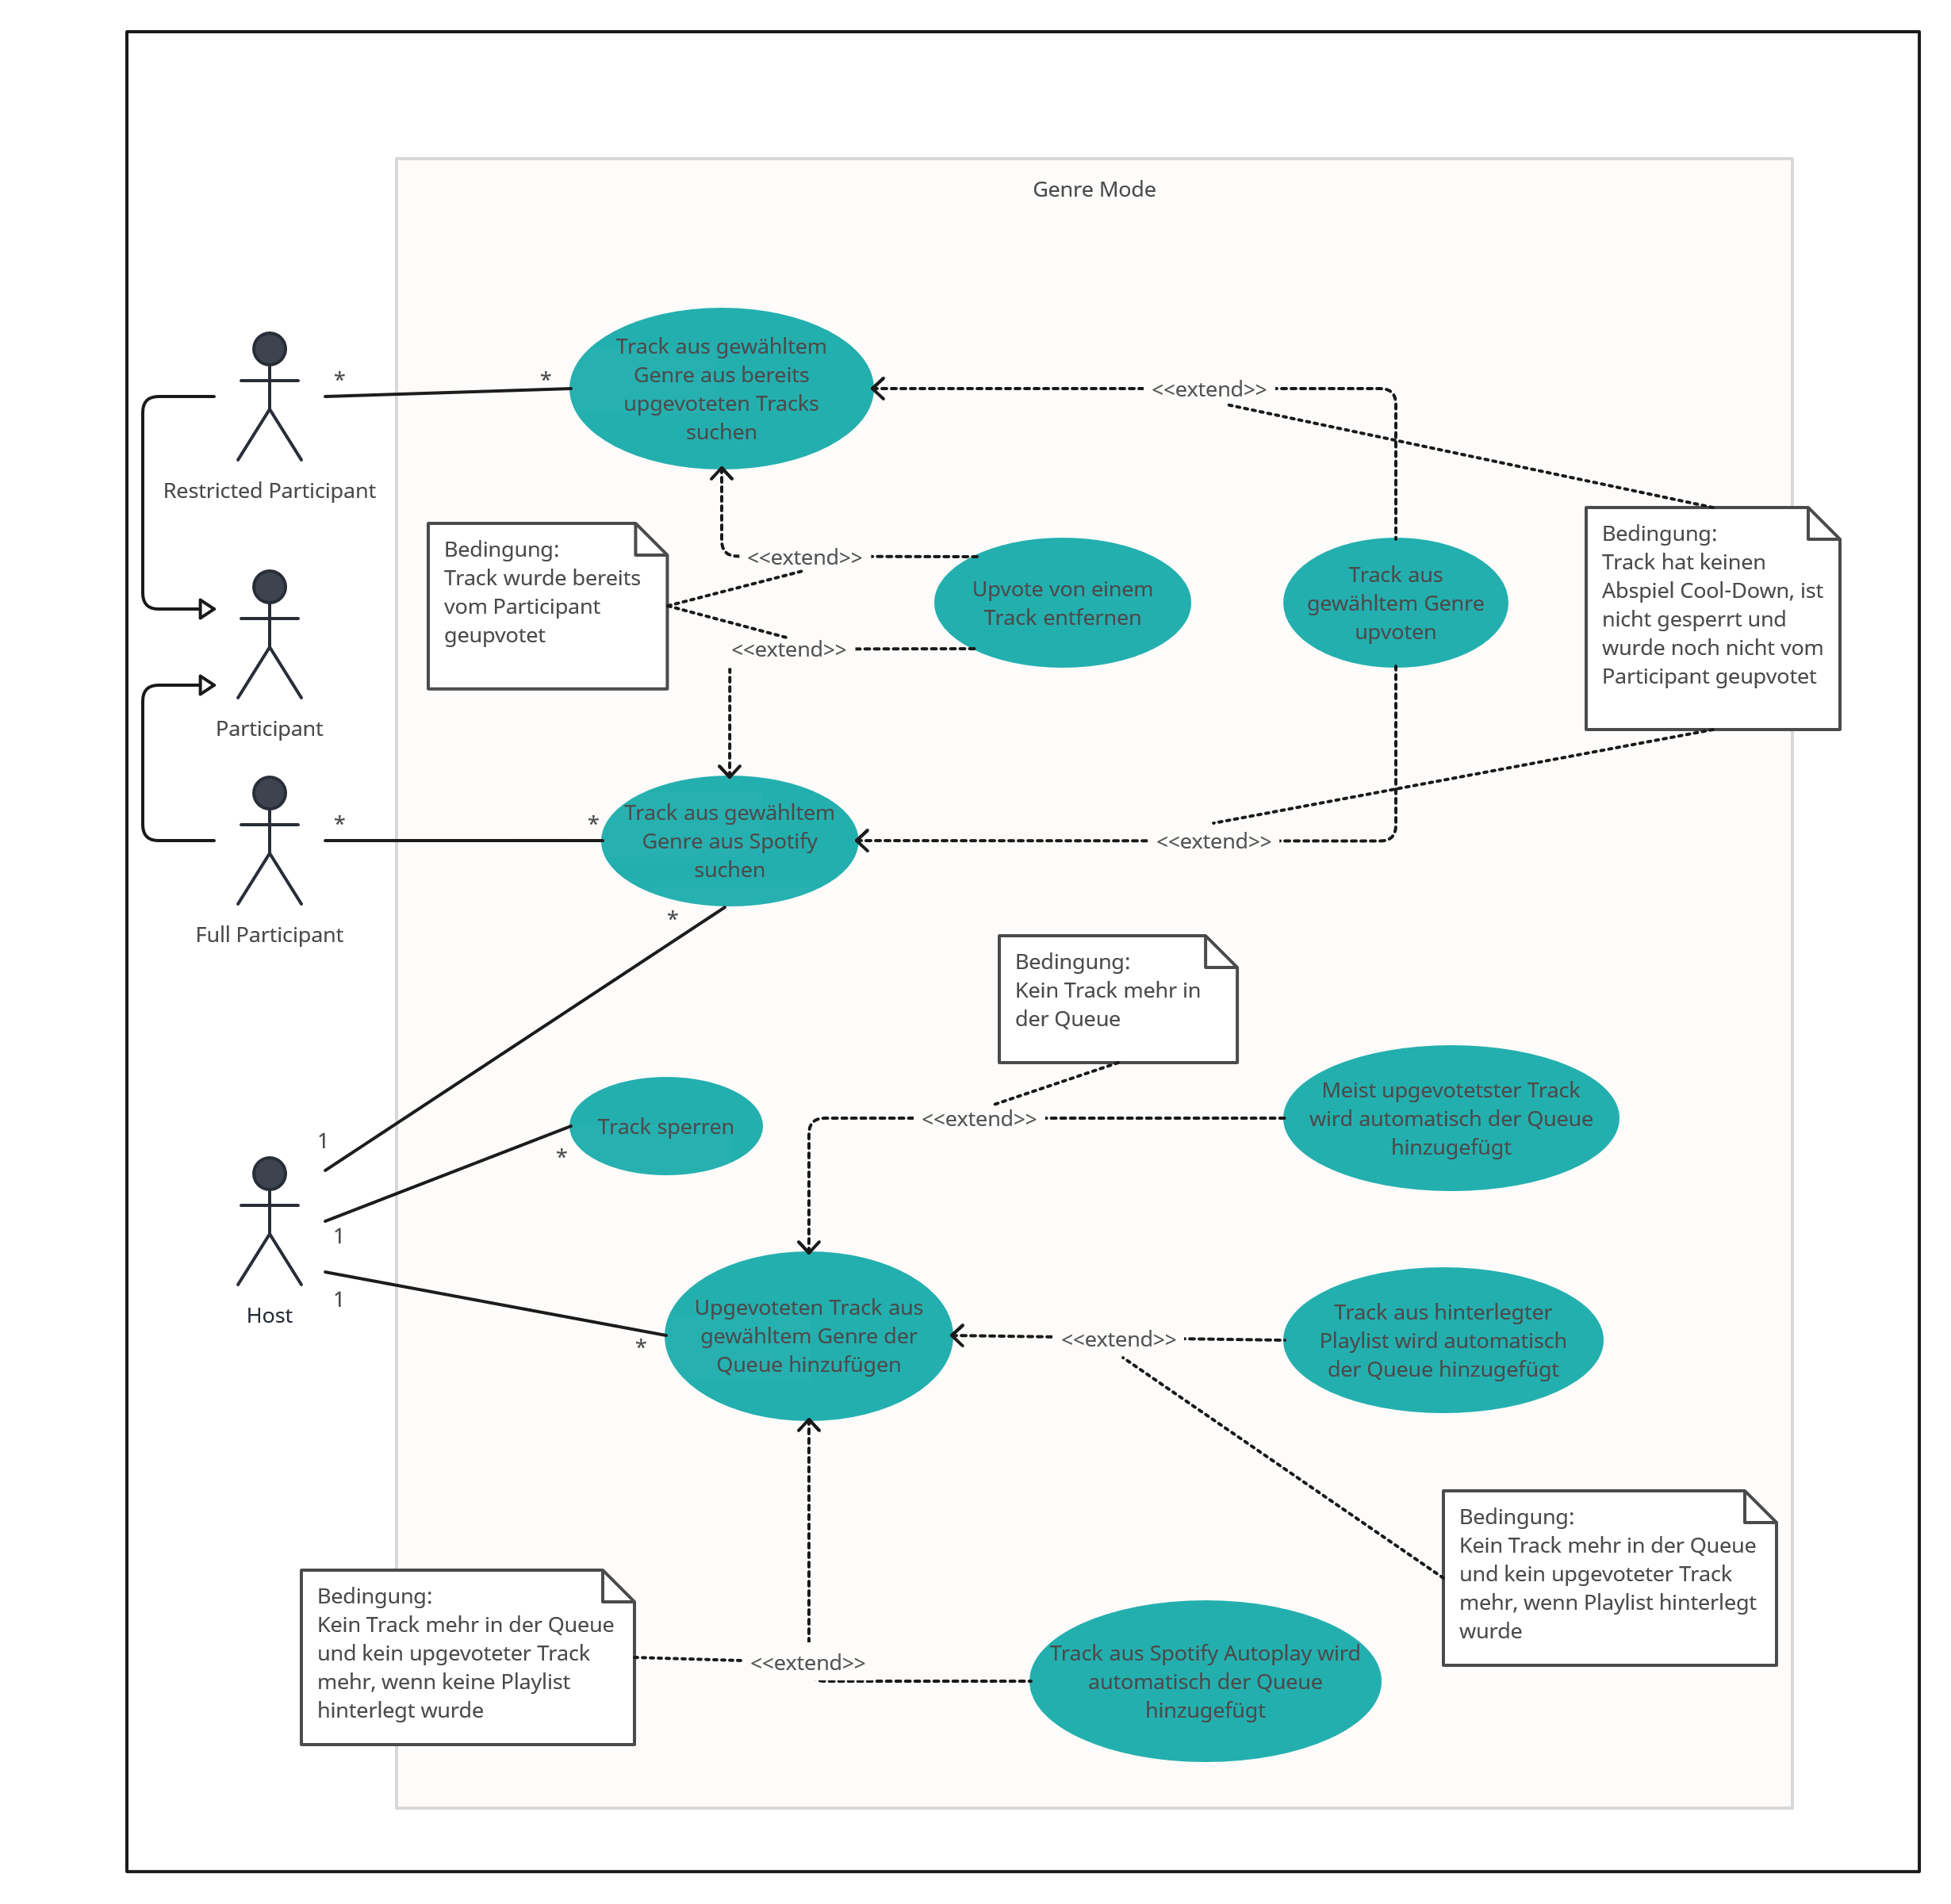
\includegraphics[width = 16cm]{LATEX/Pflichtenheft/GraphicDesigns/Use Case Genre Mode.png}
    \caption{Genre Mode}
    \label{fig:Use Case Genre Mode}
\end{figure}

\newpage

\section{Playlist Mode}
\label{sec:Anwendungsfälle:Playlist Mode}

\begin{figure}[h]
    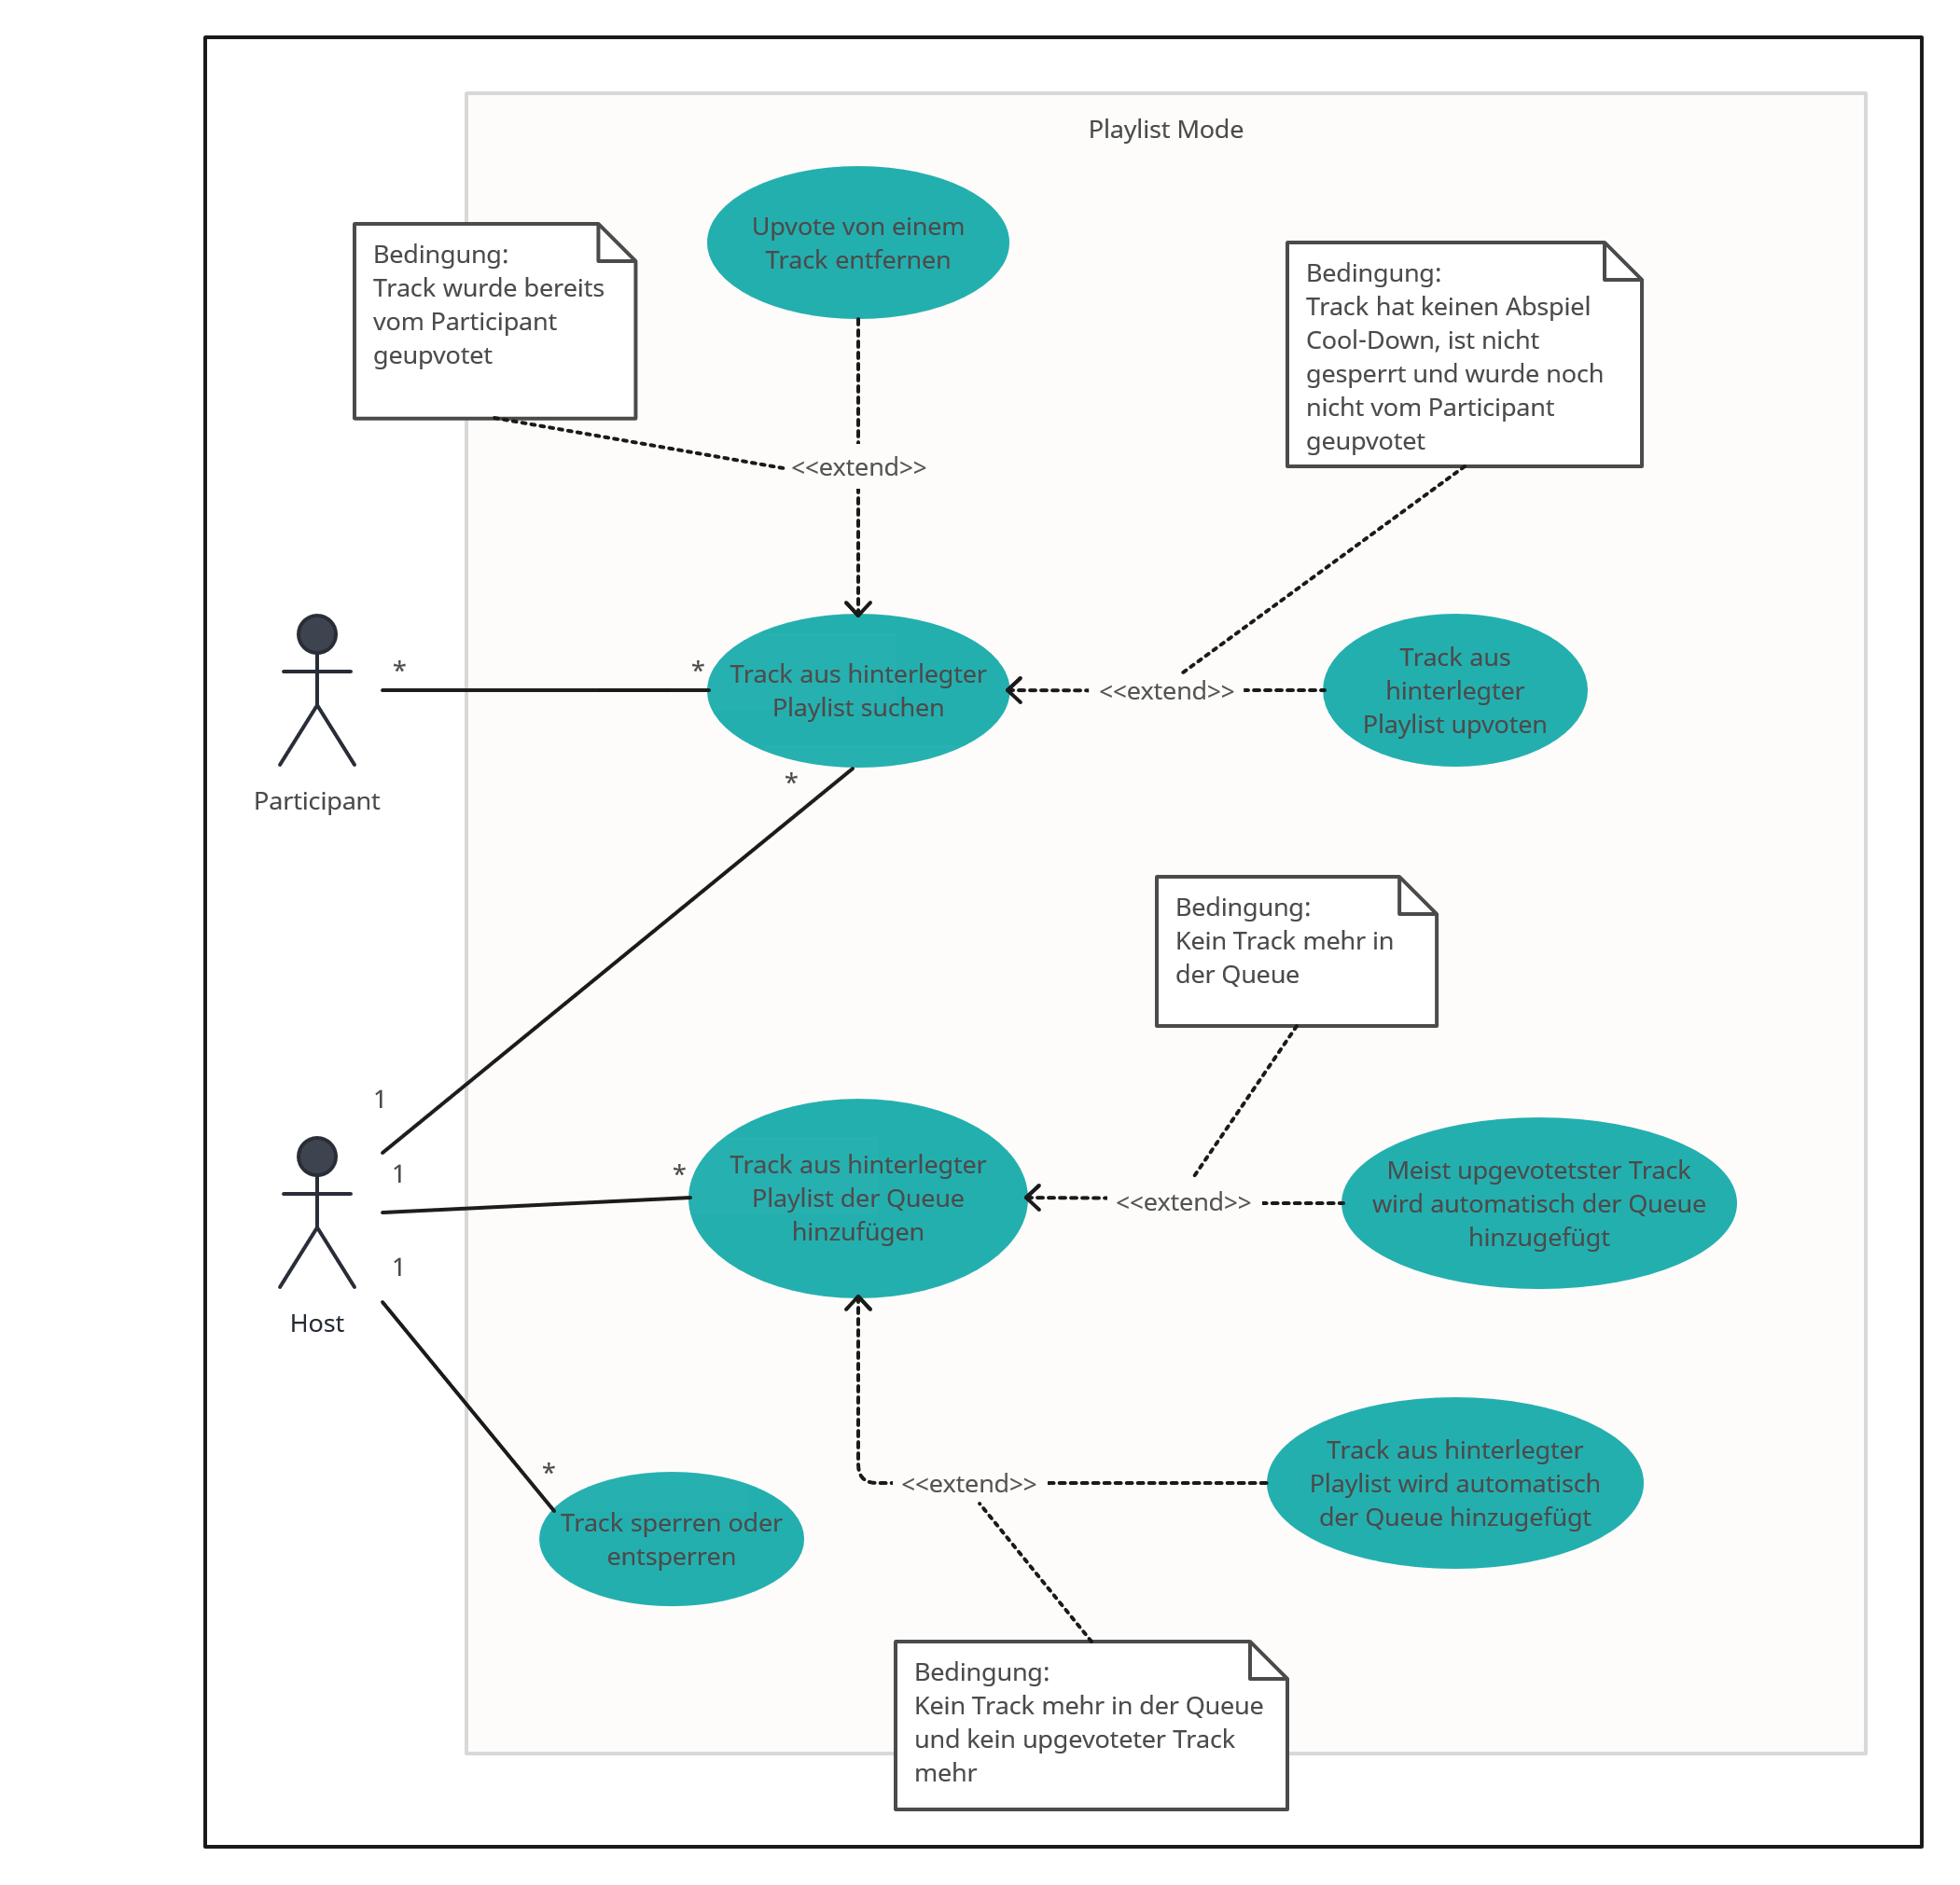
\includegraphics[width = 16cm]{LATEX/Pflichtenheft/GraphicDesigns/Use Case Playlist Mode.png}
    \caption{Playlist Mode}
    \label{fig:Use Case Playlist Mode}
\end{figure}



\chapter{Testfälle und -szenarien}
\label{chap:Tests}

In diesem Kapitel werden alle Testfälle und -szenarien definiert, die durch einen oder mehrere Benutzer des Produkts durchgeführt werden können. Die hier definierten Testfälle sollen deshalb explizit keine technischen Funktionalitäten testen, die ausreichend detailliert erst während der Entwurfsphase festgelegt werden. Solche technischen Funktionalitäten werden durch Unittests abgedeckt, die während der Entwurfs- und Implementierungsphase entworfen und implementiert werden.

\section{Testfälle}
\label{sec:Tests:Testfälle}

Testfälle sind Tests zu aus Usersicht atomaren Vorgängen. Jeder Testfall bezieht sich also auf eine einzelne atomare Usereingabe. Eine solche Usereingabe besteht entweder aus einem einzelnen Touch-Eingabe oder einer inhaltlich sehr stark zusammenhängenden Folge von Touch-Eingaben, die als atomar betrachtet wird. Falls ein Testfall nur für eine bestimmte Gruppe von Usern ausführbar ist, steht das in Klammern hinter dem Testfall mit folgenden verwendeten Abkürzungen: Host (H), Participant (P), Full Participant (FP) und Restricted Participant (RP).

\begin{enumerate}
    \item Starten und Laden der App
    \item Verlassen der App
    \item Beenden der App
    \item Beginnen des Sessionbeitrittsvorgangs
    \item Verlassen des Sessionbeitrittsvorgangs
    \item Eingabe des Zugangscodes zum Sessionbeitritt
    \item Bestätigung des Zugangscodes zum Sessionbeitritt
    \item Verlassen der Session (P)
    \item Upvote für einen Track
    \item Entfernen des Upvote von einem Track
    \item Öffnen der Tracksuche (H, FP)
    \item Verlassen der Tracksuche (H, FP)
    \item Suchen eines Tracks (FP)
    \item Vorschlagen eines Track durch Upvote (FP)
    \item Beginnen der Sessionerstellung (H)
    \item Verlassen der Sessionerstellung in der Modus-Wahl (H)
    \item Wahl des Modus (H)
    \item Zurückgehen in der Sessionerstellung von den Modus-Details zur Modus-Wahl (H)
    \item Auswählen der Details des Modus (H)
    \begin{itemize}
        \item Auswählen der Artists / der Genres / der Playlist (je nach Modus)
        \item Einstellen des Cool-Downs, wann ein Lied erneut vorgeschlagen werden kann
    \end{itemize}
    \item Bestätigung der Details des Modus (H)
    \item Löschen der Session (H)
    \item Löschen eines Tracks aus der Queue (H)
    \item Einfügen eines Tracks in die Queue aus der Tracksuche (H)
    \item Einfügen eines Tracks in die Queue aus der Vorschlagsliste (H)
    \item Ändern der Reihenfolge der Queue durch Drag and Drop (H)
    \item Löschen eines Tracks aus der Vorschlagsliste (H)
    \item Sperren eines Tracks (H) (Machen wir das überhaupt ???)
\end{enumerate}

\section{Grundlegende Testszenarien}
\label{sec:Tests:GrundlegendeTestszenarien}
\addtocontents{toc}{\protect\setcounter{tocdepth}{1}}

Grundlegende Testszenarien sind eine überschaubare und besonders essentielle Folge von atomaren Testfällen, die eine Benutzerinteraktion durchspielen. Sie setzen sich aus Testfällen oder bereits zuvor definierten grundlegenden Testszenarien zusammen.

\subsection{Grundlegendes Testszenario 1 (G1): Erstellen einer Session}
\label{subsec:Tests:GrundlegendeTestszenarien:G1}
Ein User erstellt eine Session mit einem bestimmten Modus und wird so zu ihrem Host.
\begin{itemize}
    \item Starten und Laden der App
    \item Beginnen der Sessionerstellung
    \item Wahl des Modus
    \item Auswählen der Details des Modus
    \item Bestätigung der Details des Modus
\end{itemize}


\subsection{Grundlegendes Testszenario 2 (G2): Beitritt einer Session als Full Participant}
\label{subsec:Tests:GrundlegendeTestszenarien:G2}
Ein User, tritt als Full Participant einer Session mit einem bestimmten Modus bei, die von einem anderen User als Host erstellt wurde.
Dazu muss bereits G1 (\ref{subsec:Tests:GrundlegendeTestszenarien:G1}) abgelaufen sein.
\begin{itemize}
    \item Starten und Laden der App
    \item Beginnen des Sessionbeitrittsvorgangs
    \item Eingabe des Zugangscodes zum Sessionbeitritt
    \item Bestätigung des Zugangscodes zum Sessionbeitritt
\end{itemize}


\subsection{Grundlegendes Testszenario 3 (G3): Beitritt einer Session als Passive Participant}
\label{subsec:Tests:GrundlegendeTestszenarien:G3}
Ein User, tritt als Restricted Participant einer Session mit einem bestimmten Modus bei, die von einem anderen User als Host erstellt wurde.
Dazu muss bereits G1 (\ref{subsec:Tests:GrundlegendeTestszenarien:G1}) abgelaufen sein.
\begin{itemize}
    \item Starten und Laden der App
    \item Beginnen des Sessionbeitrittsvorgangs
    \item Eingabe des Zugangscodes zum Sessionbeitritt
    \item Bestätigung des Zugangscodes zum Sessionbeitritt
\end{itemize}

\subsection{Grundlegendes Testszenario 4 (G4): Vorschlagen eines Songs als Full Participant}
\label{subsec:Tests:GrundlegendeTestszenarien:G4}
Ein User, der schon als Full Particpant einer Session mit einem bestimmten Modus beigetreten ist, die von einem anderen User als Host erstellt wurde, schlägt einen Song vor, indem er ihn zum ersten Mal upvotet. \\
Dazu muss bereits G1 (\ref{subsec:Tests:GrundlegendeTestszenarien:G1}) und dann G2 (\ref{subsec:Tests:GrundlegendeTestszenarien:G2}) abgelaufen sein.
\begin{itemize}
    \item Öffnen der Songsuche
    \item Suchen eines Songs
    \item Vorschlagen eines Songs
\end{itemize}

\subsection{Grundlegendes Testszenario 5 (G5): Vorschlagen eines Songs als Host}
\label{subsec:Tests:GrundlegendeTestszenarien:G5}
Der Host schlägt einen Song vor, indem er ihn zum ersten Mal upvotet. \\
Dazu muss bereits G1 (\ref{subsec:Tests:GrundlegendeTestszenarien:G1}) abgelaufen sein.
\begin{itemize}
    \item Öffnen der Songsuche
    \item Suchen eines Songs
    \item Vorschlagen eines Songs
\end{itemize}

\subsection{Grundlegendes Testszenario 6 (G6): Upvoten eines Songs}
\label{subsec:Tests:GrundlegendeTestszenarien:G6}
Ein User in einer Session mit einem bestimmten Modus votet einen Song up. \\
Dazu muss bereits G1 (\ref{subsec:Tests:GrundlegendeTestszenarien:G1}) und dann G2 oder G3 (\ref{subsec:Tests:GrundlegendeTestszenarien:G2} oder \ref{subsec:Tests:GrundlegendeTestszenarien:G3}) und dann G4 (\ref{subsec:Tests:GrundlegendeTestszenarien:G4}) abgelaufen sein.
\begin{itemize}
    \item Upvote für einen Song
\end{itemize}

\subsection{Grundlegendes Testszenario 7 (G7): Hinzufügen eines bestimmten vorgeschlagenen Tracks zur Queue}
\label{subsec:Tests:GrundlegendeTestszenarien:G7}
Der Host fügt einen bestimmten Track aus der Vorschlagsliste in einer Session mit einem bestimmten Modus zur Queue hinzu.
Dazu muss bereits G1 (\ref{subsec:Tests:GrundlegendeTestszenarien:G1}) abgelaufen sein.
\begin{itemize}
    \item Einfügen eines Tracks in die Queue aus der Vorschlagsliste
\end{itemize}

\subsection{Grundlegendes Testszenario 8 (G8): Vollständiges Beenden einer Session}
\label{subsec:Tests:GrundlegendeTestszenarien:G8}
Alle Participants verlassen die Session, anschließend beendet der Host die Session. Alle User verlassen und beenden die App.
Dazu muss bereits mindestens G1 (\ref{subsec:Tests:GrundlegendeTestszenarien:G1}) abgelaufen sein.
\begin{itemize}
    \item Alle Participants der Session: Verlassen der Session
    \item Löschen der Session (Host)
    \item Alle User (Participants und Host): Verlassen der App
    \item Alle User (Participants und Host): Beenden der App
\end{itemize}


\addtocontents{toc}{\protect\setcounter{tocdepth}{2}}
\section{Erweiterte Testszenarien}
\label{sec:Tests:ErweiterteTestszenarien}
\addtocontents{toc}{\protect\setcounter{tocdepth}{1}}

Erweiterte Testszenarien sind eine nicht-essentielle und möglicherweise längere Folge von atomaren Testfällen, die eine Benutzerinteraktion durchspielen. Sie setzen sich aus Testfällen und grundlegenden Testszenarien zusammen.


\subsection{Erweitertes Testszenario 1 (E1): Grundlegende Session-Funktionalität}
\label{subsec:Tests:ErweiterteTestszenarien:E1}
Ein Host (H) erstellt eine Session, der ein Full Participant (FP) beitritt. Anschließend wird die Session ordnungsgemäß beendet und alle User beenden die App.
\begin{itemize}
    \item G1 (H)
    \item G2 (FP)
    \item G8
\end{itemize}


\subsection{Erweitertes Testszenario 2 (E2): Track-Upvote und Abspielen}
\label{subsec:Tests:ErweiterteTestszenarien:E1}
Ein Host (H) erstellt eine Session, der ein Full Participant (FP) und ein Restricted Partipant (RP) beitreten. FP schlägt einen Song vor durch Upvote, den auch RP upvotet und H dann in die Queue hinzufügt.
\begin{itemize}
    \item G1 (H)
    \item G2 (FP)
    \item G3 (RP)
    \item G4 (FP)
    \item G6 (RP)
    \item G7 (H)
\end{itemize}


\subsection{Erweitertes Testszenario 3 (E3): Abspielen von fünf vorgeschlagenen Tracks}
\label{subsec:Tests:ErweiterteTestszenarien:E3}
Ein Host (H) erstellt eine Session, der ein Full Participant (FP) und zwei Restricted Partipants (R1 und R2) beitreten. H schlägt zwei Tracks vor, FP schlägt Tracks Songs vor. R1 votet einen Track von H und einen Track von FP up. R2 votet nur denselben Track von H up. H spielt die Tracks nach Anzahl der Upvotes ab.
\begin{itemize}
    \item G1 (H)
    \item G2 (FP)
    \item G3 (R1)
    \item G3 (R2)
    \item G4 (FP) (3x)
    \item G5 (H) (2x)
    \item G6, Song von H (R1)
    \item G6, Song von FP (R1)
    \item G6, selber Song von H (R2)
    \item G7 (H) (5x, in Reihenfolge der Upvotes)
\end{itemize}


\addtocontents{toc}{\protect\setcounter{tocdepth}{2}}
\chapter{Entwicklungsumgebung}
\label{chap:Entwicklungsumgebung}

\section{Software}
\label{sec:Entwicklungsumgebung:Software}

\begin{itemize}
    \item Entwicklung
    \begin{itemize}
        \item Android Studio Giraffe (2022.3.1)
    \end{itemize}
    
    \item Versionsverwaltung
    \begin{itemize}
        \item Git
        \item GitHub (zur Kommunikation)
    \end{itemize}

    \item UML Modellierung
    \begin{itemize}
        \item Creately
    \end{itemize}

    \item Grafikentwürfe
    \begin{itemize}
        \item PHPStorm
        \item GIMP
    \end{itemize}

    \item Sonstige Software
    \begin{itemize}
        \item Overleaf (für LATEX Dokumentation)
    \end{itemize}
    
\end{itemize}

\section{Hardware}
\label{sec:Entwicklungsumgebung:Hardware}

\begin{itemize}
    \item Diverse handelsübliche PCs und Laptops
    \item Diverse Android Smartphones mit mindestens Android 7.0
    \item Linux Rootserver
\end{itemize}


\chapter{Begriffserklärungen}
\label{chap:Begriffserklärungen}

\textbf{App}
 - Der Teil des Softwaresystems, der auf dem Android-Gerät des Nutzers läuft.

 \textbf{Full Participant}
 - Mit dem Musikdienst verknüpfter Participant, der Tracks im gesamten Katalog des Musikdienstes suchen kann.

\textbf{Host}
 - Ersteller einer Session, der (vorgeschlagene) Musik abspielt (kein Participant). Der Host benötigt ein Premium Abonnenment des Musikdienstes Spotify.

 \textbf{Musikdienst}
 - Der Musik-Streaminganbieter, über den die App Musik abspielt. Bei dieser App ist das Spotify.

 \textbf{Participant}
 - Teilnehmer einer Session (nicht der Host). Überbegriff für Full Participant und Restricted Participant.

 \textbf{Produkt}
 - Der Zustand, in dem das System nach Fertigstellung sein wird.

 \textbf{Queue}
 - Liste von Liedern, welche als nächstes durch den Musikdienst abgespielt werden.

 \textbf{Restricted Participant}
 - Nicht mit dem Musikdienst verknüpfter Participant, der nur Tracks von den bisher upgevoteten suchen kann.

 \textbf{Server}
 - Der Teil des Softwaresystems, der nicht auf dem Android-Gerät des Nutzers, sondern auf einem zentralen und externen Server läuft.

 \textbf{Session}
 - Eine Gruppe aus Participants und einem Host. In ihr können Tracks upgevotet und vom Host abgespielt werden.

\textbf{System}
 - Das gesamte zu entwickelnde Softwaresystem, Überbegriff von App und Server.

 \textbf{Track}
 - Lied bzw. Musikstück.

 \textbf{Upvote}
 - Bewertung auf einen Track. Je mehr Upvotes ein Track hat, desto beliebter ist er.

 \textbf{User}
 - Jeder Benutzer der App, Participant und Host sind User.

 \textbf{Vorschlagsliste}
 - Liste von Tracks einer Session, die mindestens ein Upvote haben.
 

\end{document}
